\chapter{KẾT QUẢ ỨNG DỤNG}
\label{ch:results}

\section{Đặc tả Yêu cầu Phần mềm (SRS)}
\label{sec:srs}

\subsection{Mô tả tổng quan}
\label{subsec:overall_description}

PerFin là ứng dụng mobile quản lý tài chính cá nhân với giao diện hội thoại AI (chatbot) làm trung tâm. Ứng dụng cho phép người dùng ghi chép giao dịch thông qua nhiều phương thức nhập liệu (văn bản, giọng nói, hình ảnh), tự động phân loại và phân tích chi tiêu bằng AI, quản lý ngân sách, theo dõi dòng tiền đa tài khoản, và nhận tư vấn tài chính cá nhân hóa.

\textbf{Đối tượng người dùng mục tiêu:}
\begin{itemize}
    \item Sinh viên, người đi làm trẻ (18--35 tuổi) muốn quản lý tài chính cá nhân nhưng ngại các ứng dụng truyền thống phức tạp.
    \item Người dùng thích giao tiếp bằng ngôn ngữ tự nhiên hơn là điền biểu mẫu.
\end{itemize}

\textbf{Các tác nhân chính (Actors):}

\begin{table}[htbp]
\centering
\begin{tabularx}{\textwidth}{|l|X|}
\hline
\textbf{Actor} & \textbf{Mô tả} \\ \hline
\textbf{User} & Người dùng cuối quản lý tài chính cá nhân \\ \hline
\textbf{AI Engine} & Hệ thống AI xử lý NLP, OCR, Voice-to-Text, phân loại tự động \\ \hline
\textbf{System} & Hệ thống backend tự động (cron jobs, notifications, encryption) \\ \hline
\textbf{Admin/Reviewer} & Quản trị viên duyệt dữ liệu, quản lý danh mục hệ thống và nhân cách AI \\ \hline
\end{tabularx}
\caption{Các tác nhân trong hệ thống}
\label{tab:actors}
\end{table}

\subsection{Yêu cầu cụ thể}
\label{subsec:specific_requirements}

Hệ thống PerFin được phân tách thành 9 nhóm yêu cầu chính (Requirements), mỗi nhóm đặc tả chi tiết trong tài liệu REQ riêng biệt:

\begin{table}[htbp]
\centering
\begin{tabularx}{\textwidth}{|l|l|X|}
\hline
\textbf{Mã REQ} & \textbf{Tên yêu cầu} & \textbf{Mô tả tóm tắt} \\ \hline
REQ-01 & Nhập liệu đa phương thức bằng AI & Ghi chép giao dịch bằng chat văn bản, giọng nói, hoặc hình ảnh. AI tự động bóc tách dữ liệu. \\ \hline
REQ-02 & Phân loại thông minh & Tự động phân loại giao dịch vào danh mục dựa trên ngữ cảnh, học từ phản hồi người dùng. \\ \hline
REQ-03 & Quản lý Ngân sách & Thiết lập hạn mức chi tiêu, theo dõi tiến độ, cảnh báo chủ động, rollover. \\ \hline
REQ-04 & Phân tích và Báo cáo cá nhân hóa & Biểu đồ trực quan, phát hiện bất thường, tư vấn AI cá nhân hóa. \\ \hline
REQ-05 & Quản lý Tài khoản đa nguồn & Quản lý nhiều ví/tài khoản, chuyển tiền giữa ví, tính tài sản ròng. \\ \hline
REQ-06 & Phân tách Dòng tiền \& Tài sản & Tracking đầu tư, phân biệt Transfer/Investment/Expense, Net Worth, dòng tiền. \\ \hline
REQ-07 & Xuất Dữ liệu \& Sao lưu & Xuất CSV/PDF, sao lưu mã hóa, khôi phục dữ liệu, sao lưu tự động. \\ \hline
REQ-08 & Quản lý Chi phí Cố định \& Nhắc nhở & Chi phí định kỳ, AI nhận diện chu kỳ, nhắc nhở thanh toán, lịch sử thanh toán. \\ \hline
REQ-09 & Nhân cách AI & Phong cách giao tiếp đa dạng, gamification, behavioral psychology. \\ \hline
\end{tabularx}
\caption{Danh sách các yêu cầu hệ thống}
\label{tab:requirements}
\end{table}

\subsection{Yêu cầu chức năng}
\label{subsec:functional_requirements}

\subsubsection{REQ-01: Nhập liệu đa phương thức bằng AI}
\textbf{Tóm tắt:} Cho phép người dùng tạo giao dịch thu/chi mới thông qua giao diện hội thoại bằng văn bản tự nhiên, tin nhắn thoại hoặc hình ảnh. Hệ thống sử dụng AI để đọc hiểu đầu vào tiếng Việt, tiếng Anh hoặc câu pha trộn Việt - Anh; bóc tách tên giao dịch và giá tiền; suy đoán danh mục tương ứng; hỏi lại khi thiếu thông tin.

\textit{Chi tiết đầy đủ: xem phụ lục \ref{sec:appendix_req01}.}

\subsubsection{REQ-02: Phân loại thông minh}
\textbf{Tóm tắt:} Dựa trên ngữ cảnh chat hoặc nội dung hóa đơn, hệ thống tự động phân loại giao dịch vào đúng danh mục. Hỗ trợ danh mục mặc định, danh mục tùy chỉnh, danh mục con, và học từ phản hồi người dùng.

\textit{Chi tiết đầy đủ: xem phụ lục \ref{sec:appendix_req02}.}

\subsubsection{REQ-03: Quản lý Ngân sách}
\textbf{Tóm tắt:} Cho phép thiết lập hạn mức chi tiêu theo danh mục hoặc tổng thể trong kỳ tuần/tháng. Hệ thống tự động theo dõi tiến độ chi tiêu, cảnh báo chủ động tại ngưỡng 70\%, 90\%, 100\%, hỗ trợ rollover ngân sách chưa dùng hết.

\textit{Chi tiết đầy đủ: xem phụ lục \ref{sec:appendix_req03}.}

\subsubsection{REQ-04: Phân tích và Báo cáo cá nhân hóa}
\textbf{Tóm tắt:} Hệ thống tổng hợp dữ liệu giao dịch thành biểu đồ trực quan và đưa ra nhận xét, tư vấn bằng AI dựa trên thói quen chi tiêu thực tế của người dùng. Phát hiện xu hướng bất thường và đưa ra gợi ý cải thiện.

\textit{Chi tiết đầy đủ: xem phụ lục \ref{sec:appendix_req04}.}

\subsubsection{REQ-05: Quản lý Tài khoản đa nguồn}
\textbf{Tóm tắt:} Cho phép tạo và quản lý nhiều ví/tài khoản tài chính (tiền mặt, ngân hàng, ví điện tử, đầu tư). Hỗ trợ chuyển tiền giữa các ví (Transfer), tính tài sản ròng (Net Worth), gán giao dịch vào ví bằng chat.

\textit{Chi tiết đầy đủ: xem phụ lục \ref{sec:appendix_req05}.}

\subsubsection{REQ-06: Phân tách Dòng tiền \& Tài sản}
\textbf{Tóm tắt:} Tracking dòng tiền đầu tư, phân biệt Transfer/Investment/Expense, tính tài sản ròng (Net Worth) chính xác. Theo dõi lãi/lỗ đầu tư cơ bản, báo cáo tổng quan dòng tiền, quản lý dòng tiền bằng chat.

\textit{Chi tiết đầy đủ: xem phụ lục \ref{sec:appendix_req06}.}

\subsubsection{REQ-07: Xuất Dữ liệu \& Sao lưu}
\textbf{Tóm tắt:} Xuất giao dịch ra CSV, xuất báo cáo ra PDF, sao lưu toàn bộ dữ liệu dưới dạng mã hóa, khôi phục dữ liệu, sao lưu tự động định kỳ, yêu cầu xuất/sao lưu qua chat.

\textit{Chi tiết đầy đủ: xem phụ lục \ref{sec:appendix_req07}.}

\subsubsection{REQ-08: Quản lý Chi phí Cố định \& Nhắc nhở}
\textbf{Tóm tắt:} Thiết lập chi phí cố định (tiền nhà, tiền điện, tiền nước...), AI tự động nhận diện chi phí cố định từ lịch sử giao dịch, nhắc nhở chủ động khi đến hạn thanh toán, xác nhận và ghi nhận thanh toán, tạm dừng/kích hoạt lại, theo dõi lịch sử thanh toán.

\textit{Chi tiết đầy đủ: xem phụ lục \ref{sec:appendix_req08}.}

\subsubsection{REQ-09: Nhân cách AI}
\textbf{Tóm tắt:} Chatbot áp dụng các phong cách giao tiếp khác nhau (Chuyên gia tài chính, Bà mẹ nghiêm khắc, Bạn thân, Huấn luyện viên). Mỗi nhân cách ảnh hưởng đến giọng điệu và cách đưa ra lời khuyên nhưng không thay đổi logic xử lý giao dịch.

\textit{Chi tiết đầy đủ: xem phụ lục \ref{sec:appendix_req09}.}

\subsection{Yêu cầu phi chức năng}
\label{subsec:non_functional_requirements}

\begin{table}[htbp]
\centering
\begin{tabularx}{\textwidth}{|l|l|X|}
\hline
\textbf{\#} & \textbf{Yêu cầu} & \textbf{Mô tả} \\ \hline
NFR-01 & Ngôn ngữ & Hệ thống hỗ trợ tiếng Việt, tiếng Anh và câu pha trộn Việt - Anh. \\ \hline
NFR-02 & Hiệu năng & Thời gian phản hồi chat $\le$ 3 giây cho xử lý văn bản, $\le$ 8 giây cho OCR. \\ \hline
NFR-03 & Bảo mật & Mã hóa dữ liệu at-rest (AES-256) và in-transit (TLS 1.2+). JWT cho xác thực. \\ \hline
NFR-04 & Khả dụng & Uptime $\ge$ 99\% cho dịch vụ core (không tính downtime API bên ngoài). \\ \hline
NFR-05 & Khả năng mở rộng & Kiến trúc microservice, có thể scale horizontal từng service. \\ \hline
NFR-06 & Tương thích & Hỗ trợ Android 8.0+ và iOS 14.0+. \\ \hline
NFR-07 & Dữ liệu per-user & Tất cả dữ liệu tài chính là riêng tư, chỉ người sở hữu mới có quyền truy cập. \\ \hline
NFR-08 & Độ chính xác AI & Tỷ lệ phân loại danh mục chính xác $\ge$ 85\% cho danh mục mặc định. \\ \hline
NFR-09 & Sao lưu & Hỗ trợ sao lưu tự động và khôi phục dữ liệu hoàn toàn. \\ \hline
NFR-10 & Xuất dữ liệu & Hỗ trợ xuất CSV và PDF với định dạng chuẩn. \\ \hline
\end{tabularx}
\caption{Các yêu cầu phi chức năng}
\label{tab:nfr}
\end{table}



\section{Thiết kế Phần mềm}
\label{sec:software_design}

\subsection{Kiến trúc ứng dụng (Application Architecture)}
\label{subsec:app_architecture}

PerFin được xây dựng theo kiến trúc phân tầng (Layered Architecture) kết hợp microservice, bao gồm 5 tầng chính:
\begin{enumerate}
    \item \textbf{Tầng Client (Mobile App):} Giao diện người dùng trên mobile, bao gồm Chat UI, Transaction UI, Report UI, Settings UI.
    \item \textbf{Tầng API Gateway:} Điểm vào duy nhất cho mọi yêu cầu từ client, xử lý rate limiting, routing, kiểm tra xác thực.
    \item \textbf{Tầng Dịch vụ Lõi (Core Services):} Các service nghiệp vụ chính --- Auth, Transaction, Category, Budget, Reminder, Export, Backup, Report, Notification.
    \item \textbf{Tầng Dịch vụ AI:} AI Service điều phối các engine con --- NLP Engine, OCR Engine, Voice-to-Text, Categorization Engine, Personality Engine.
    \item \textbf{Tầng Dữ liệu:} Cơ sở dữ liệu chính (PostgreSQL/MongoDB) và Object Storage (S3) cho ảnh, exports, backups.
\end{enumerate}

\begin{figure}[htbp]
    \centering
    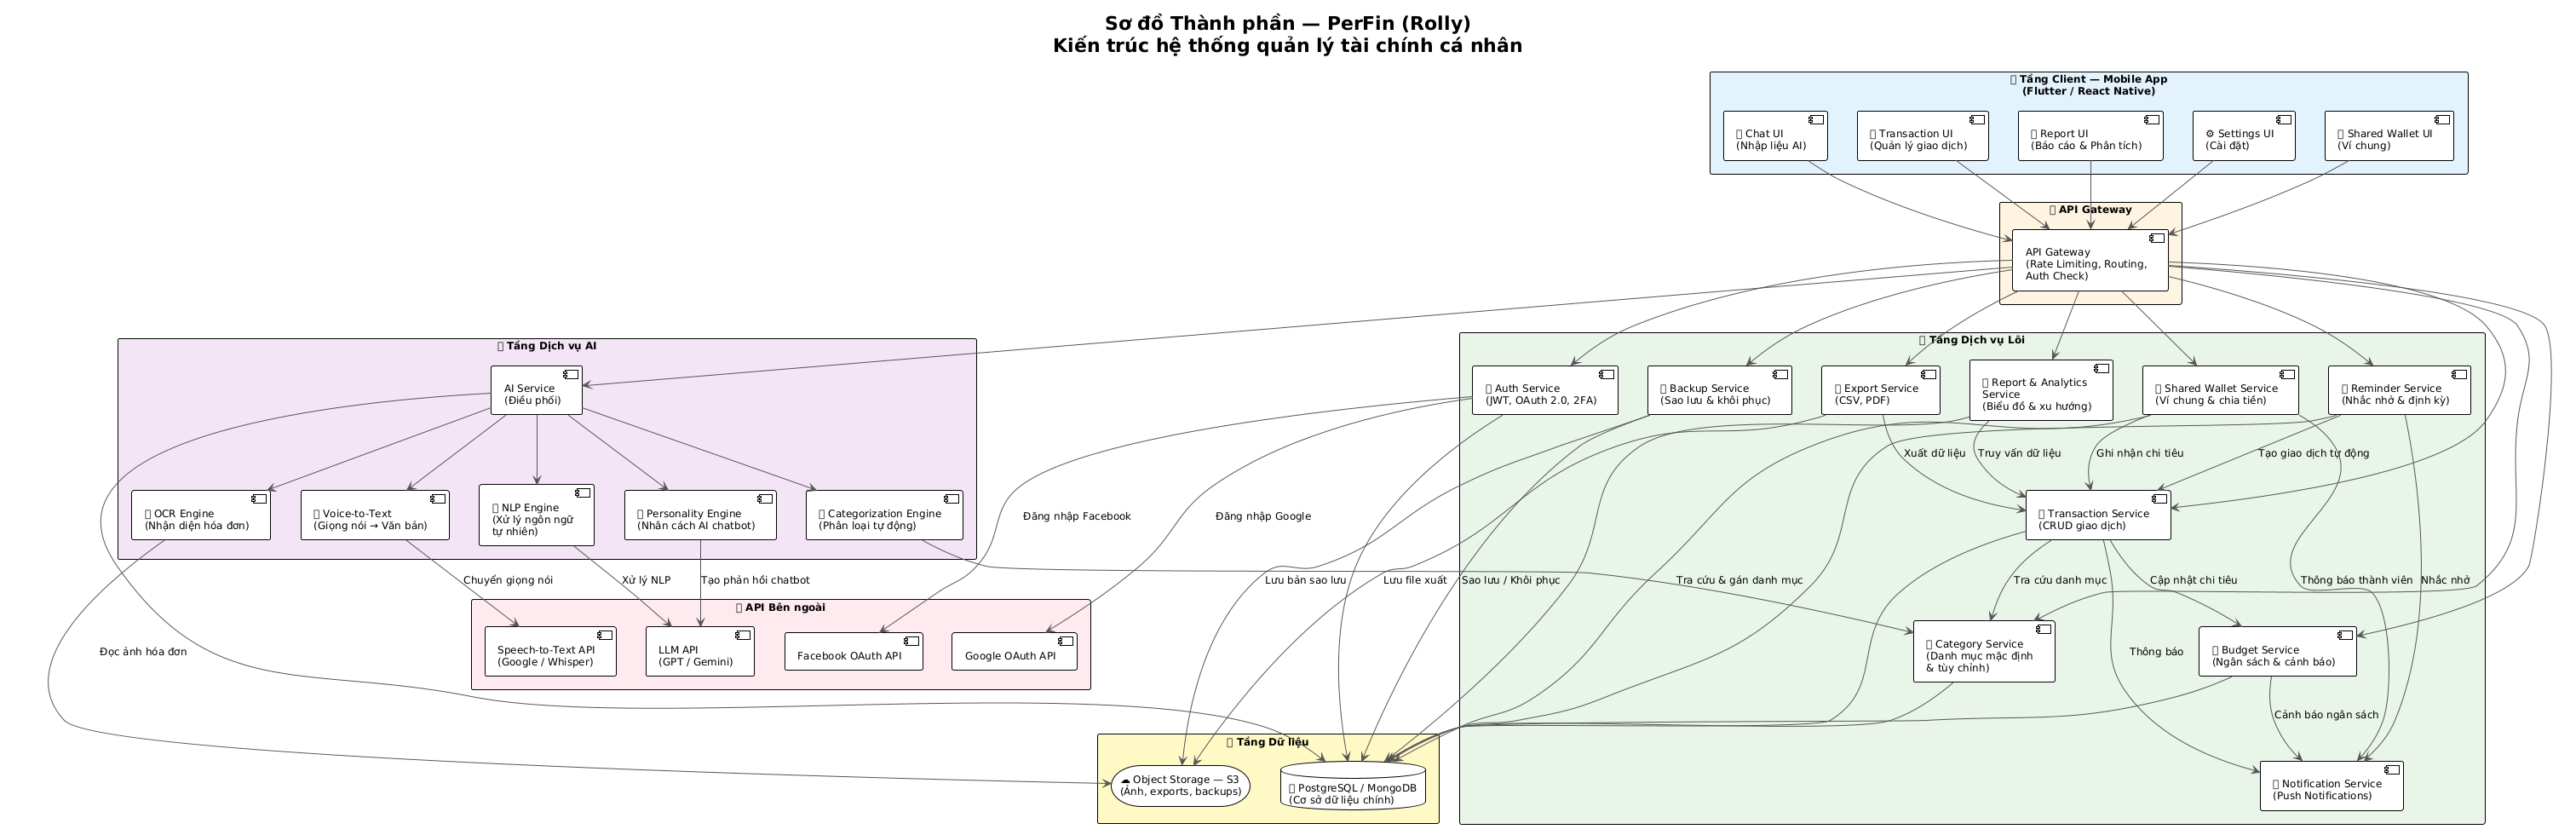
\includegraphics[width=\textwidth]{images/component-diagram.png}
    \caption{Sơ đồ thành phần (Component Diagram)}
    \label{fig:component_diagram}
\end{figure}

Dưới đây là mô tả chi tiết vai trò và trách nhiệm của từng tầng trong kiến trúc hệ thống:

\begin{itemize}
    \item \textbf{Tầng Client (Mobile App):} Ứng dụng Flutter đa nền tảng (Android/iOS) đóng vai trò là giao diện tương tác trực tiếp với người dùng. Tầng này bao gồm các module giao diện chính: \textit{Chat UI} (giao diện hội thoại với AI --- màn hình trung tâm), \textit{Transaction UI} (quản lý và xem danh sách giao dịch), \textit{Report UI} (biểu đồ và báo cáo chi tiêu), \textit{Budget UI} (thiết lập và theo dõi ngân sách), \textit{Wallet UI} (quản lý ví/tài khoản), và \textit{Settings UI} (cài đặt ứng dụng, nhân cách AI). Flutter cho phép dùng chung codebase cho cả hai nền tảng, giảm chi phí phát triển và đảm bảo trải nghiệm đồng nhất.

    \item \textbf{Tầng API Gateway:} Đóng vai trò là điểm vào duy nhất (single entry point) cho mọi yêu cầu HTTP từ phía client. API Gateway thực hiện các chức năng: \textit{routing} (điều phối yêu cầu đến đúng service xử lý), \textit{rate limiting} (giới hạn số lượng yêu cầu nhằm chống lạm dụng), \textit{JWT validation} (xác minh token xác thực trước khi chuyển tiếp yêu cầu), và \textit{request/response transformation} (chuẩn hóa định dạng dữ liệu). Việc tập trung các chức năng cross-cutting tại Gateway giúp các service phía sau tập trung vào logic nghiệp vụ.

    \item \textbf{Tầng Dịch vụ Lõi (Core Services):} Bao gồm các service xử lý nghiệp vụ chính của ứng dụng, mỗi service đảm nhận một miền chức năng riêng biệt: \textit{Auth Service} (đăng ký, đăng nhập, quản lý phiên JWT, OAuth 2.0), \textit{Transaction Service} (CRUD giao dịch, tính toán số dư), \textit{Category Service} (quản lý danh mục mặc định và tùy chỉnh), \textit{Budget Service} (thiết lập hạn mức, theo dõi tiến độ, kiểm tra ngưỡng cảnh báo), \textit{Wallet Service} (quản lý ví, chuyển tiền, tính Net Worth), \textit{Reminder Service} (nhắc nhở định kỳ, chi phí cố định), \textit{Export Service} (xuất CSV/PDF), \textit{Backup Service} (sao lưu mã hóa, khôi phục), \textit{Report Service} (tổng hợp dữ liệu, phân tích xu hướng), và \textit{Notification Service} (gửi thông báo đẩy, cảnh báo trong chat).

    \item \textbf{Tầng Dịch vụ AI (AI Services):} AI Service đóng vai trò là bộ điều phối (orchestrator) cho các engine xử lý trí tuệ nhân tạo. Khi nhận được yêu cầu từ Core Services, AI Service xác định loại tác vụ và chuyển đến engine phù hợp: \textit{NLP Engine} (sử dụng Google Gemini API để phân tích ngữ nghĩa văn bản tiếng Việt, trích xuất intent và entity từ câu chat), \textit{OCR Engine} (sử dụng Google Vision API để nhận dạng văn bản từ ảnh hóa đơn), \textit{Voice-to-Text Engine} (sử dụng Google Speech-to-Text để chuyển đổi giọng nói thành văn bản), \textit{Categorization Engine} (phân loại giao dịch dựa trên ngữ cảnh và lịch sử người dùng), và \textit{Personality Engine} (áp dụng phong cách giao tiếp theo nhân cách AI đã chọn). Các engine hoạt động theo pipeline: đầu ra của engine này có thể là đầu vào của engine khác, ví dụ Voice-to-Text $\rightarrow$ NLP $\rightarrow$ Categorization.

    \item \textbf{Tầng Dữ liệu (Data Tier):} Bao gồm hai thành phần lưu trữ chính: \textit{PostgreSQL} làm cơ sở dữ liệu quan hệ chính, lưu trữ toàn bộ dữ liệu có cấu trúc (structured data) như thông tin người dùng, giao dịch, danh mục, ngân sách, ví; và \textit{Object Storage} (Firebase/Cloud Storage) lưu trữ các tệp nhị phân như ảnh hóa đơn, file xuất CSV/PDF, và bản sao lưu mã hóa. PostgreSQL được chọn vì hỗ trợ tốt các ràng buộc toàn vẹn dữ liệu (foreign key, check constraint), giao dịch ACID, và hiệu năng truy vấn phân tích với các hàm tổng hợp (aggregate functions).
\end{itemize}

\subsection{Thiết kế dữ liệu (Data Design)}
\label{subsec:data_design}

\subsubsection{Sơ đồ lớp (Class Diagram)}
Hệ thống PerFin bao gồm các thực thể (entity) chính:
\begin{itemize}
    \item \textbf{User}: Thông tin người dùng, cài đặt cá nhân.
    \item \textbf{Transaction}: Giao dịch thu/chi/đặc biệt, liên kết với Category và Wallet.
    \item \textbf{Category}: Danh mục giao dịch (mặc định và tùy chỉnh), hỗ trợ cấu trúc cha-con.
    \item \textbf{Wallet}: Ví/tài khoản tài chính (tiền mặt, ngân hàng, ví điện tử, đầu tư).
    \item \textbf{Budget}: Ngân sách theo danh mục hoặc tổng thể, với kỳ tuần/tháng.
    \item \textbf{Reminder}: Nhắc nhở giao dịch và chi phí cố định.
    \item \textbf{AIPersonality}: Nhân cách AI chatbot.
    \item \textbf{ChatMessage}: Lưu trữ lịch sử hội thoại.
\end{itemize}

\begin{figure}[htbp]
    \centering
    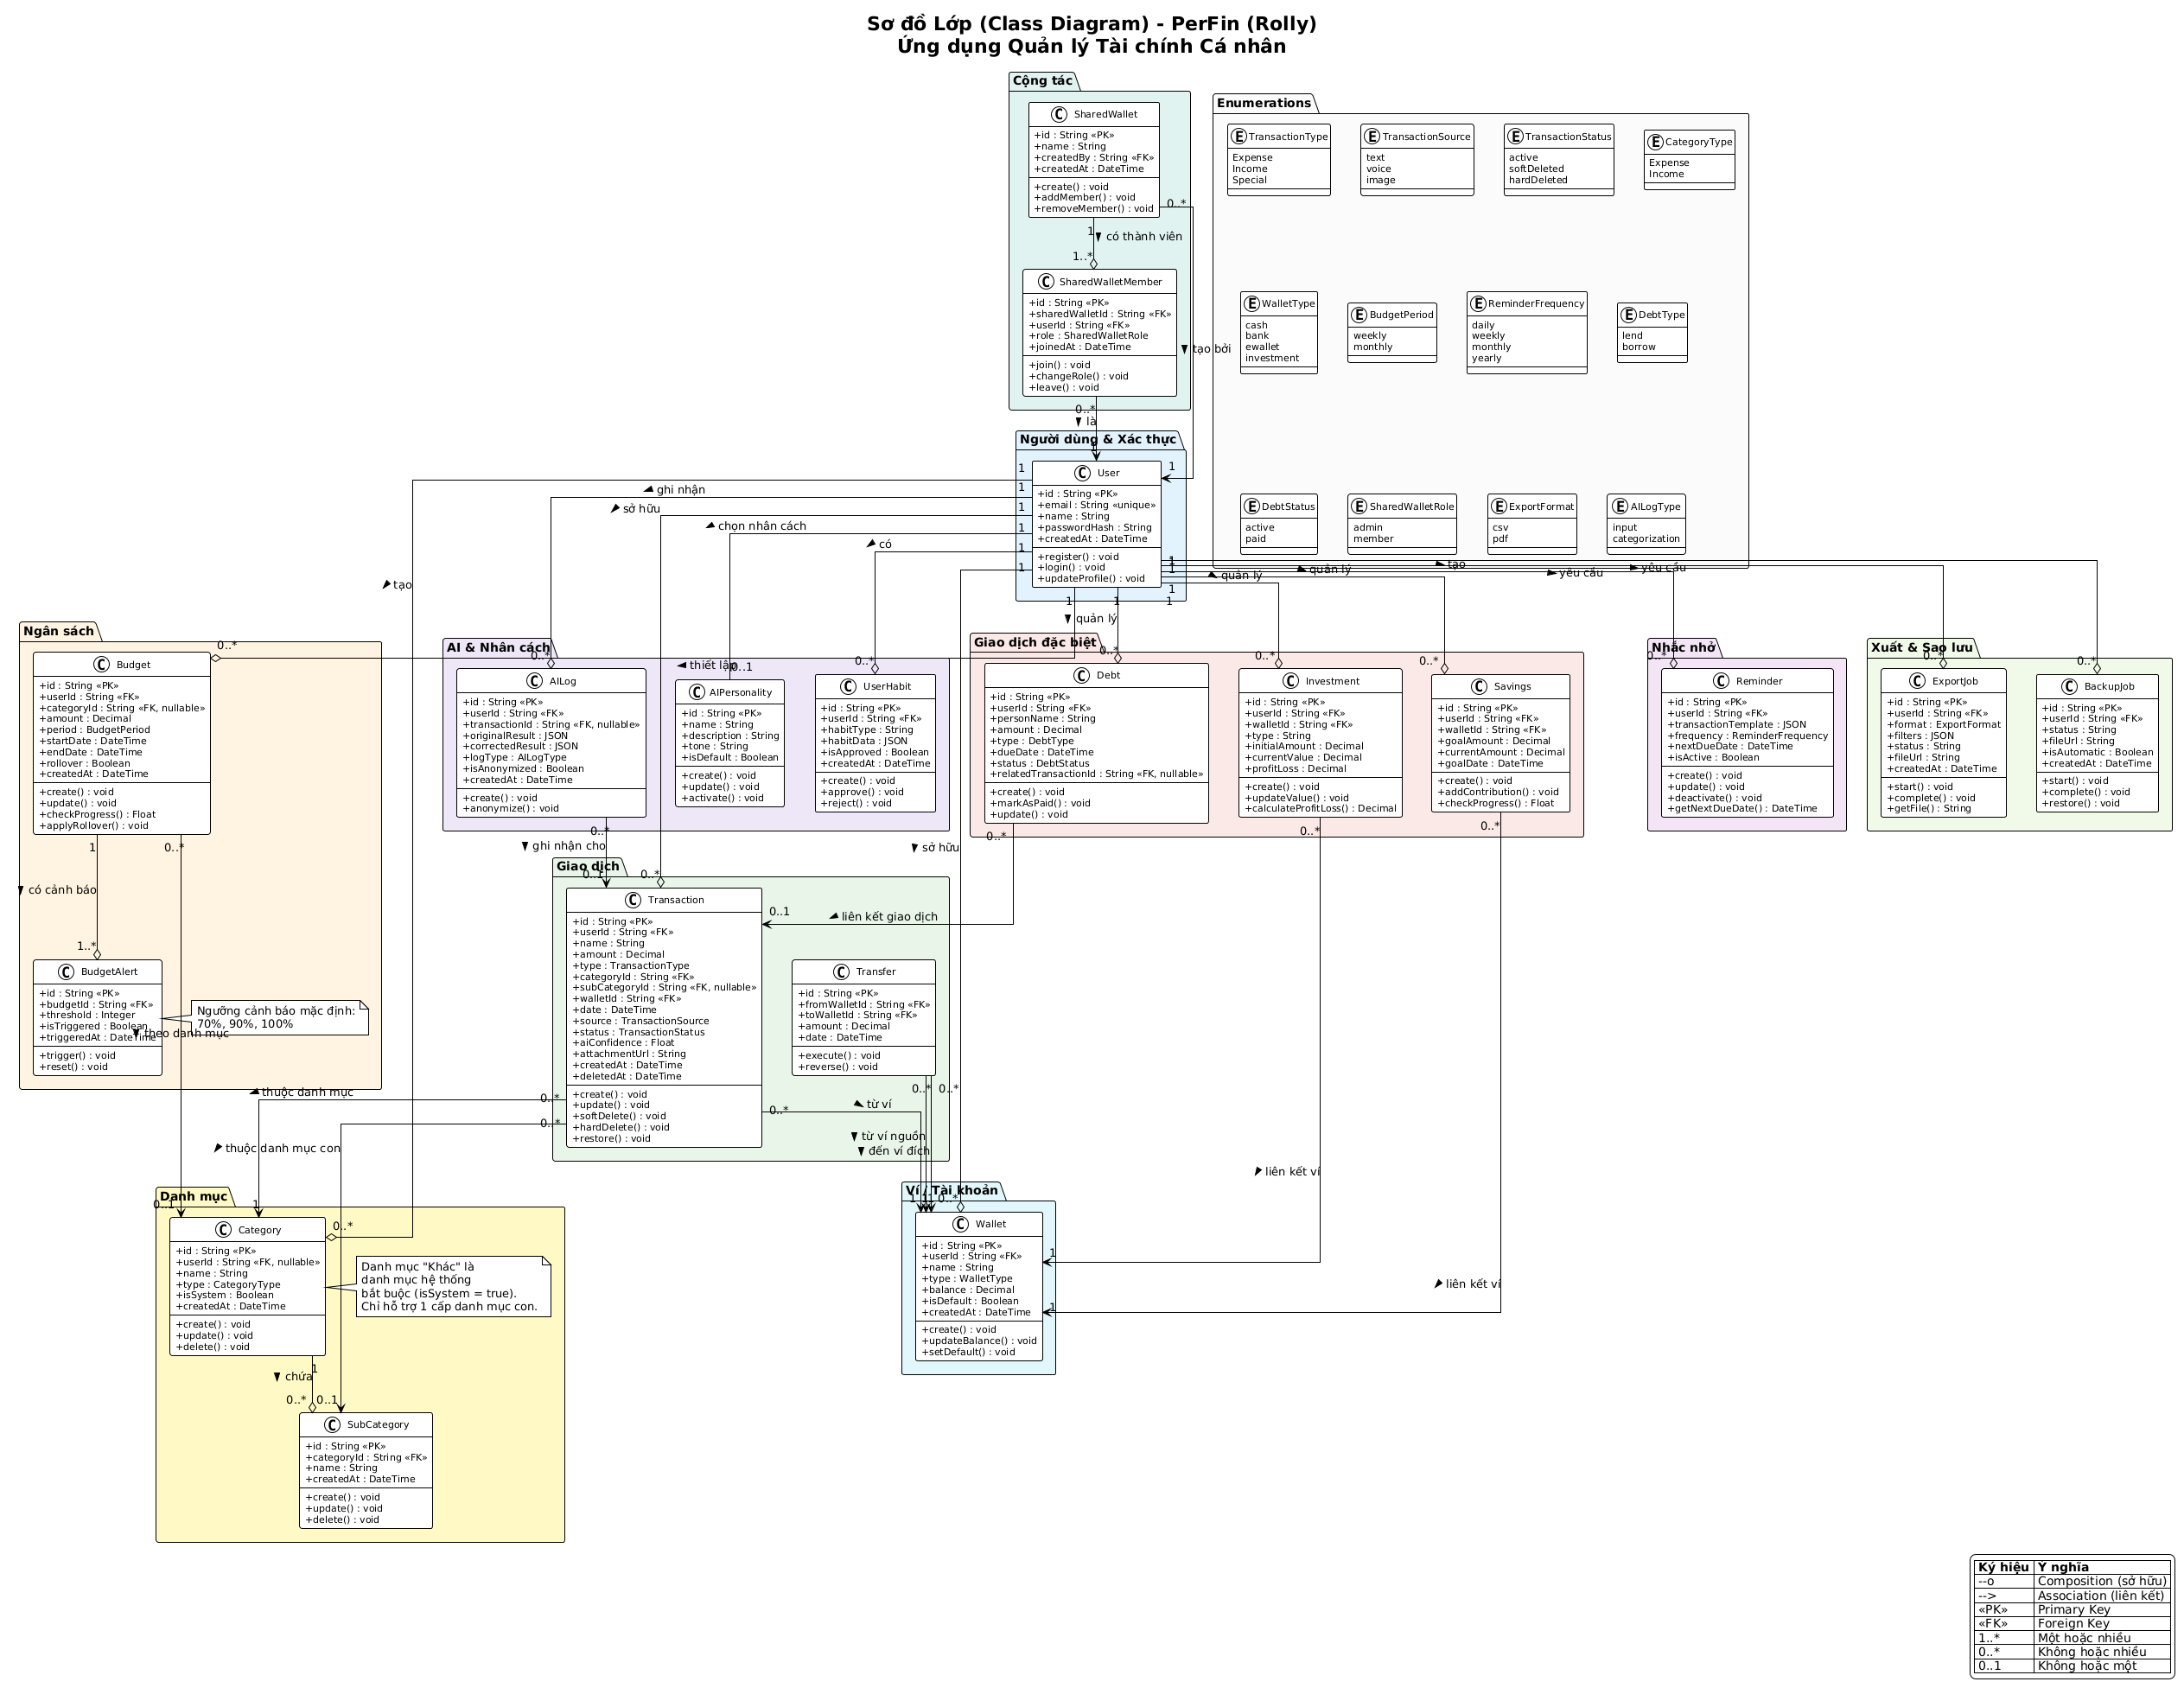
\includegraphics[width=\textwidth]{images/class-diagram.png}
    \caption{Sơ đồ lớp (Class Diagram)}
    \label{fig:class_diagram}
\end{figure}

Các quan hệ chính giữa các thực thể trong hệ thống được mô tả như sau:

\begin{itemize}
    \item \textbf{User $\leftrightarrow$ Transaction:} Quan hệ 1-n (one-to-many). Mỗi User sở hữu nhiều Transaction, mỗi Transaction thuộc về đúng một User. Đây là quan hệ cốt lõi đảm bảo tính riêng tư dữ liệu (data isolation per user).
    \item \textbf{Transaction $\leftrightarrow$ Category:} Quan hệ n-1 (many-to-one). Mỗi Transaction được gán vào một Category (do AI phân loại tự động hoặc người dùng chọn). Một Category có thể chứa nhiều Transaction.
    \item \textbf{Category $\leftrightarrow$ Category:} Quan hệ tự tham chiếu (self-referencing). Mỗi Category có thể có một parent\_category, cho phép xây dựng cấu trúc danh mục cha-con (ví dụ: ``Ăn uống'' $\rightarrow$ ``Trà sữa'', ``Cơm trưa'').
    \item \textbf{Transaction $\leftrightarrow$ Wallet:} Quan hệ n-1. Mỗi Transaction liên kết với một Wallet, cho phép theo dõi số dư từng ví. Giao dịch chuyển tiền (Transfer) liên kết với hai Wallet (nguồn và đích).
    \item \textbf{User $\leftrightarrow$ Wallet:} Quan hệ 1-n. Mỗi User có thể tạo nhiều Wallet (tiền mặt, ngân hàng, ví điện tử, đầu tư).
    \item \textbf{Budget $\leftrightarrow$ Category:} Quan hệ n-1. Mỗi Budget thiết lập hạn mức chi tiêu cho một Category cụ thể (hoặc tổng thể nếu không gắn Category). Hệ thống so sánh tổng Transaction của Category trong kỳ với hạn mức Budget để đưa ra cảnh báo.
    \item \textbf{User $\leftrightarrow$ Budget:} Quan hệ 1-n. Mỗi User có thể thiết lập nhiều Budget cho các danh mục khác nhau.
    \item \textbf{User $\leftrightarrow$ Reminder:} Quan hệ 1-n. Mỗi User có thể tạo nhiều Reminder cho các chi phí cố định.
    \item \textbf{User $\leftrightarrow$ AIPersonality:} Quan hệ n-1. Mỗi User chọn một AIPersonality đang hoạt động, nhưng một AIPersonality có thể được nhiều User sử dụng.
    \item \textbf{User $\leftrightarrow$ ChatMessage:} Quan hệ 1-n. Lịch sử hội thoại được lưu trữ theo từng User, bao gồm cả tin nhắn của người dùng và phản hồi của AI.
\end{itemize}

\subsubsection{Sơ đồ quan hệ thực thể (ERD)}

\begin{figure}[htbp]
    \centering
    %\includegraphics[width=0.8\textwidth]{diagrams/erd-diagram.png}
    \fbox{\parbox{0.8\textwidth}{\centering\vspace{1.5cm} Sơ đồ thực thể quan hệ (ERD) \\ (Vẽ ERD từ Class Diagram, thêm các trường dữ liệu và kiểu dữ liệu)\vspace{1.5cm}}}
    \caption{Sơ đồ quan hệ thực thể (ERD)}
    \label{fig:erd_diagram}
\end{figure}

Sơ đồ quan hệ thực thể (ERD) được dẫn xuất trực tiếp từ Class Diagram ở trên, với việc bổ sung các thông tin cụ thể cho tầng cơ sở dữ liệu: kiểu dữ liệu cụ thể cho từng trường (VARCHAR, INTEGER, DECIMAL, TIMESTAMP, ENUM...), khóa chính (PRIMARY KEY) cho mỗi bảng, khóa ngoại (FOREIGN KEY) thể hiện các mối quan hệ giữa các thực thể, các ràng buộc toàn vẹn (NOT NULL, UNIQUE, CHECK), và chỉ mục (INDEX) cho các trường thường xuyên truy vấn. ERD sẽ được cập nhật đầy đủ sau khi hoàn thiện quá trình phát triển cơ sở dữ liệu.

\subsection{Thiết kế chi tiết (Detailed Design)}
\label{subsec:detailed_design}

\subsubsection{Sơ đồ Use Case tổng quan}
Sơ đồ Use Case mô tả tổng quan các tác nhân và chức năng chính của hệ thống PerFin, được tổ chức theo 9 nhóm yêu cầu (REQ-01 đến REQ-09).

Do sơ đồ Use Case tổng quan chứa số lượng lớn các chức năng (từ REQ-01 đến REQ-10) nên rất lớn và khó quan sát đầy đủ trên một trang tài liệu. Vì vậy, sơ đồ được chia nhỏ thành 1 sơ đồ tổng quan mức cao (hệ thống) và 3 sơ đồ chi tiết theo các nhóm chức năng:

\begin{figure}[htbp]
    \centering
    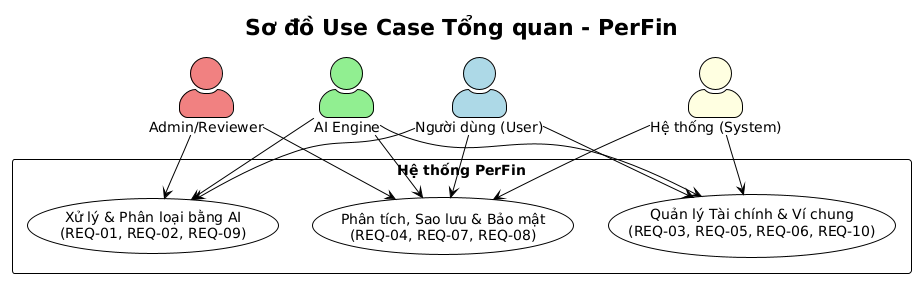
\includegraphics[width=0.9\textwidth]{images/use-case-diagram.png}
    \caption{Sơ đồ Use Case tổng quan mức cao (Overview)}
    \label{fig:use_case_overview}
\end{figure}

\begin{figure}[htbp]
    \centering
    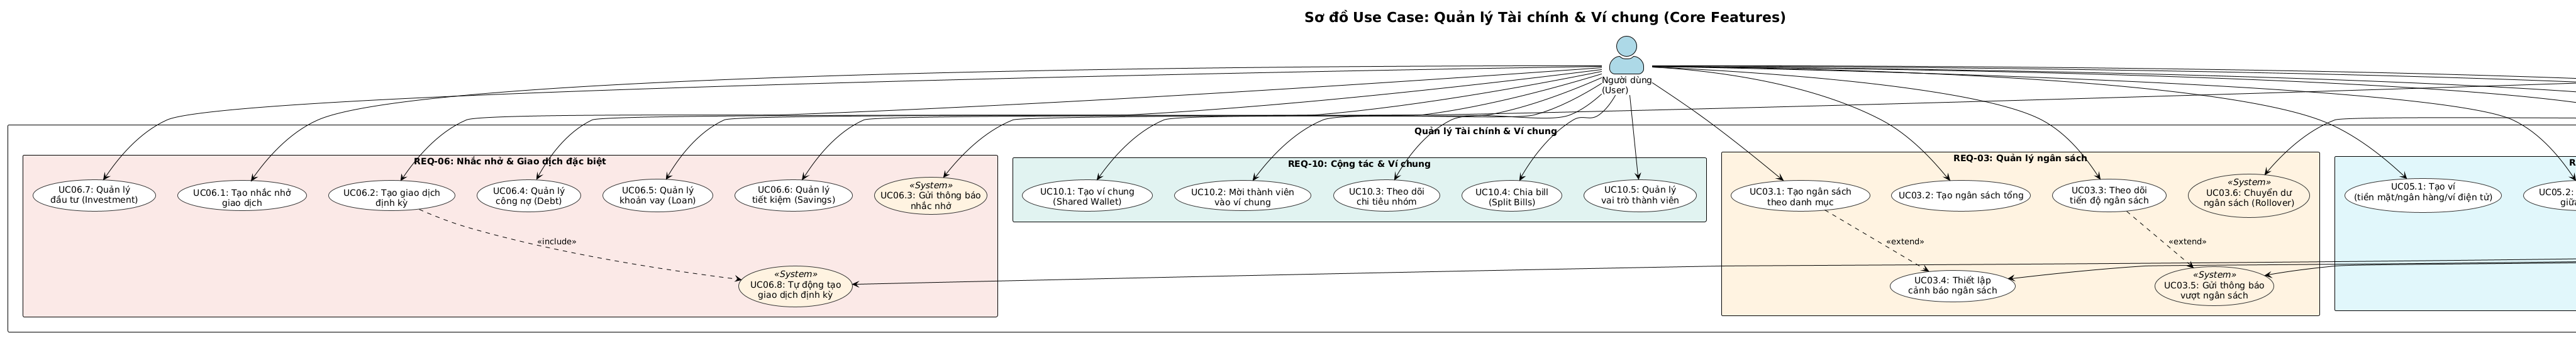
\includegraphics[width=0.95\textwidth]{images/use-case-core.png}
    \caption{Sơ đồ Use Case phân hệ Quản lý Tài chính \& Ví chung (Core Features)}
    \label{fig:use_case_core}
\end{figure}

\begin{figure}[htbp]
    \centering
    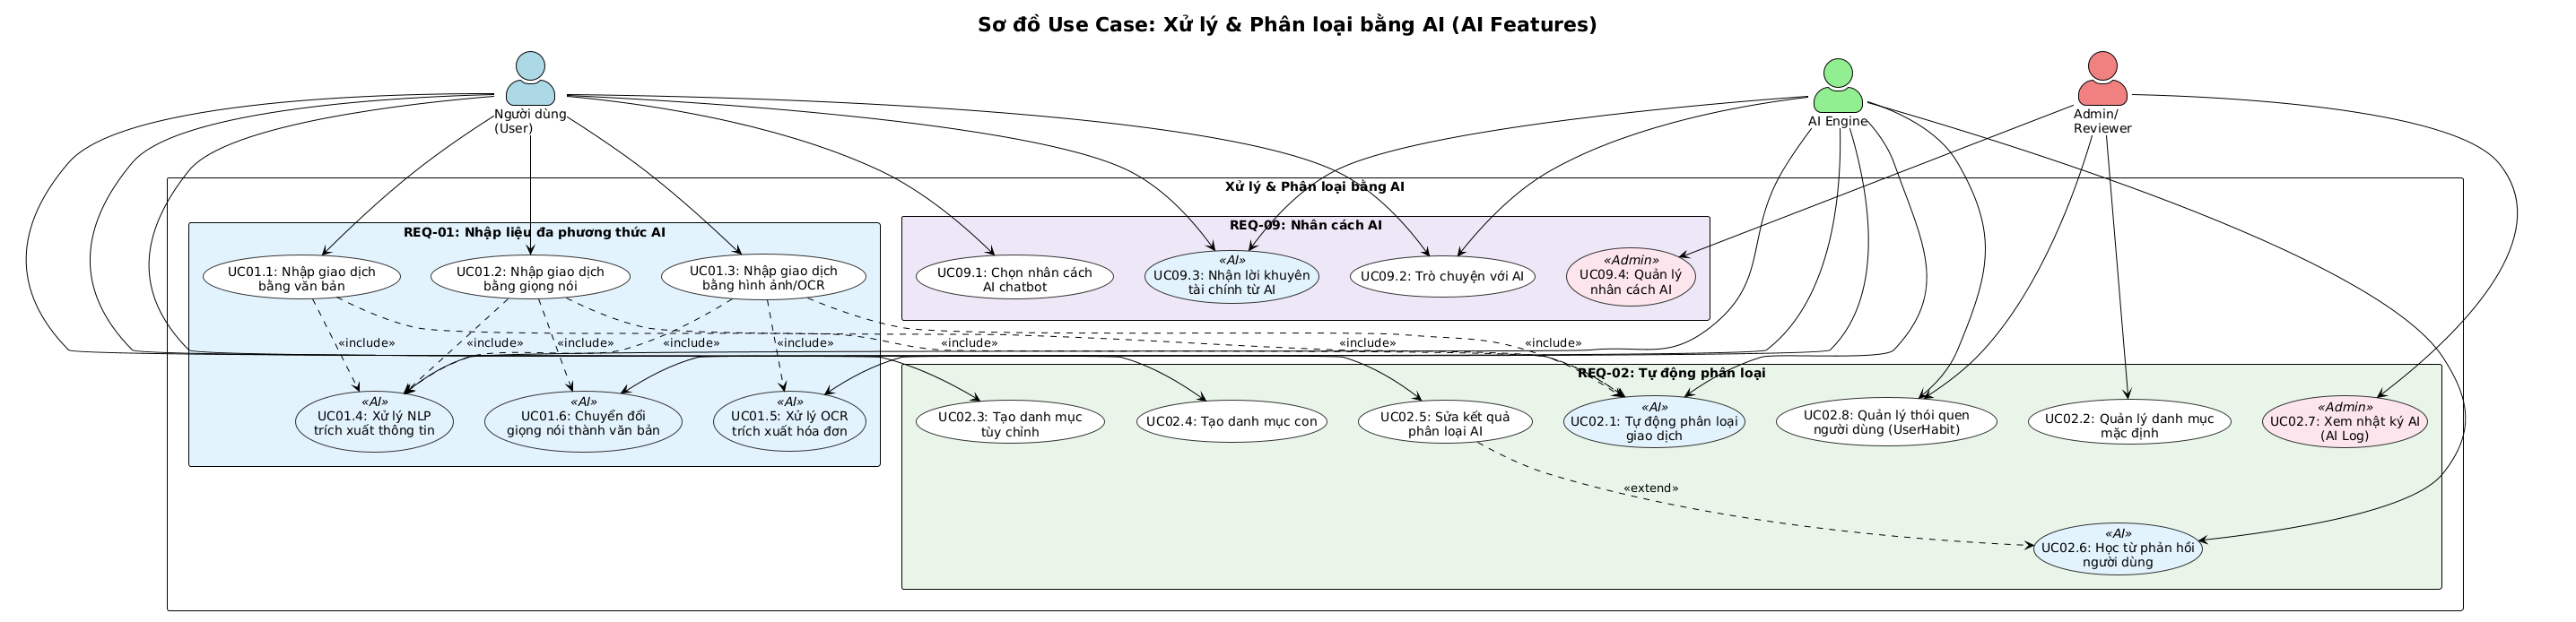
\includegraphics[width=0.95\textwidth]{images/use-case-ai.png}
    \caption{Sơ đồ Use Case phân hệ Xử lý \& Phân loại bằng AI (AI Features)}
    \label{fig:use_case_ai}
\end{figure}

\begin{figure}[htbp]
    \centering
    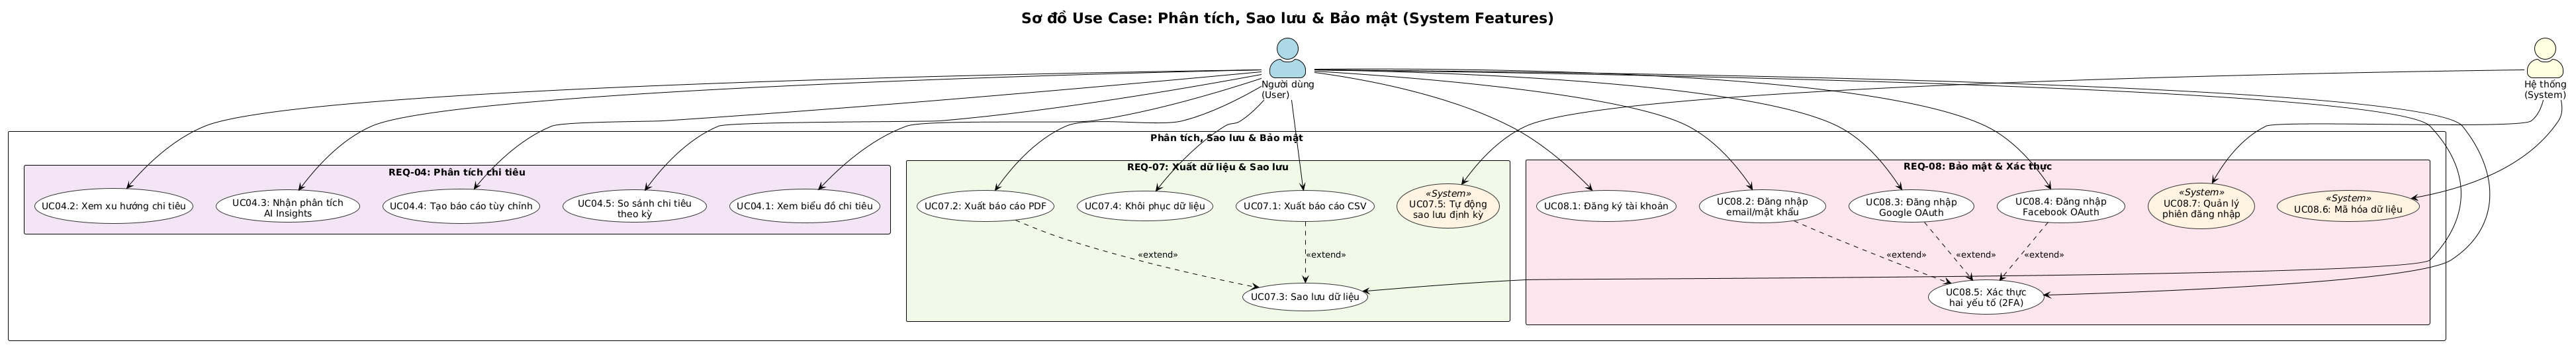
\includegraphics[width=0.95\textwidth]{images/use-case-system.png}
    \caption{Sơ đồ Use Case phân hệ Phân tích, Sao lưu \& Bảo mật (System Features)}
    \label{fig:use_case_system}
\end{figure}

Hệ thống Use Case của PerFin được tổ chức theo cấu trúc phân cấp với 4 loại tác nhân (User, AI Engine, System, Admin/Reviewer) và các use case được nhóm theo phân hệ chức năng:

\begin{itemize}
    \item \textbf{Sơ đồ tổng quan (Hình~\ref{fig:use_case_overview}):} Thể hiện mức cao các phân hệ chức năng chính và mối quan hệ giữa 4 loại actor với hệ thống. Mỗi phân hệ được biểu diễn dưới dạng một subsystem boundary, giúp người đọc nhanh chóng nắm bắt phạm vi tổng thể của ứng dụng.

    \item \textbf{Phân hệ Core Features (Hình~\ref{fig:use_case_core}):} Bao gồm các chức năng quản lý tài chính cốt lõi --- quản lý giao dịch (tạo, sửa, xóa, xem lịch sử), quản lý danh mục (tạo danh mục tùy chỉnh, cấu trúc cha-con), quản lý ngân sách (thiết lập hạn mức, theo dõi tiến độ), quản lý ví/tài khoản (tạo ví, chuyển tiền giữa các ví), và quản lý nhắc nhở (chi phí cố định, giao dịch định kỳ). Đây là phân hệ có số lượng use case lớn nhất, phản ánh tính chất ứng dụng quản lý tài chính.

    \item \textbf{Phân hệ AI Features (Hình~\ref{fig:use_case_ai}):} Tập trung vào các chức năng tích hợp trí tuệ nhân tạo --- nhập liệu thông minh (văn bản, giọng nói, ảnh hóa đơn), phân loại giao dịch tự động, phát hiện chi phí cố định từ lịch sử, và tùy chỉnh nhân cách AI. Các use case trong phân hệ này chủ yếu liên quan đến tác nhân AI Engine với các mối quan hệ \texttt{<<include>>} và \texttt{<<extend>>} phức tạp.

    \item \textbf{Phân hệ System Features (Hình~\ref{fig:use_case_system}):} Bao gồm các chức năng hỗ trợ và vận hành hệ thống --- báo cáo và phân tích chi tiêu (biểu đồ, phát hiện bất thường, tư vấn AI), sao lưu và khôi phục dữ liệu (sao lưu mã hóa, sao lưu tự động), xuất dữ liệu (CSV, PDF), và bảo mật (xác thực JWT, OAuth 2.0, mã hóa dữ liệu). Tác nhân System đóng vai trò chủ yếu trong phân hệ này với các tác vụ tự động chạy nền (background jobs).
\end{itemize}

\subsubsection{Sơ đồ tuần tự (Sequence Diagrams)}
Các sơ đồ tuần tự mô tả luồng tương tác giữa các tác nhân và hệ thống cho các use case quan trọng.

Các sơ đồ tuần tự chi tiết hóa luồng tương tác giữa các tác nhân (Người dùng, AI Engine, Hệ thống) và các dịch vụ bên trong hệ thống đối với từng nghiệp vụ cụ thể:

\begin{figure}[htbp]
    \centering
    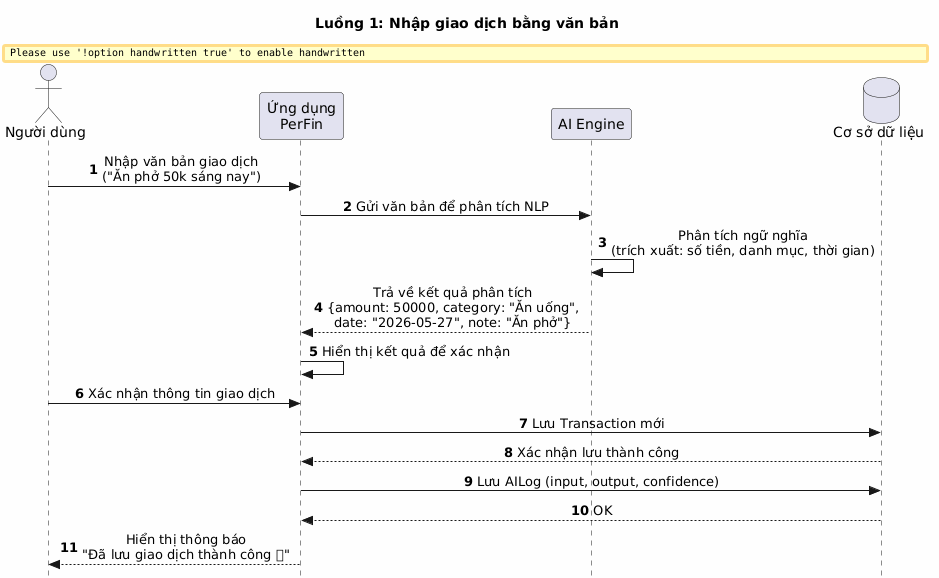
\includegraphics[width=0.9\textwidth]{images/sequence-nhập-giao-dịch-bằng-văn-bản.png}
    \caption{Sơ đồ tuần tự: Nhập giao dịch bằng văn bản}
    \label{fig:seq_text_input}
\end{figure}

\begin{figure}[htbp]
    \centering
    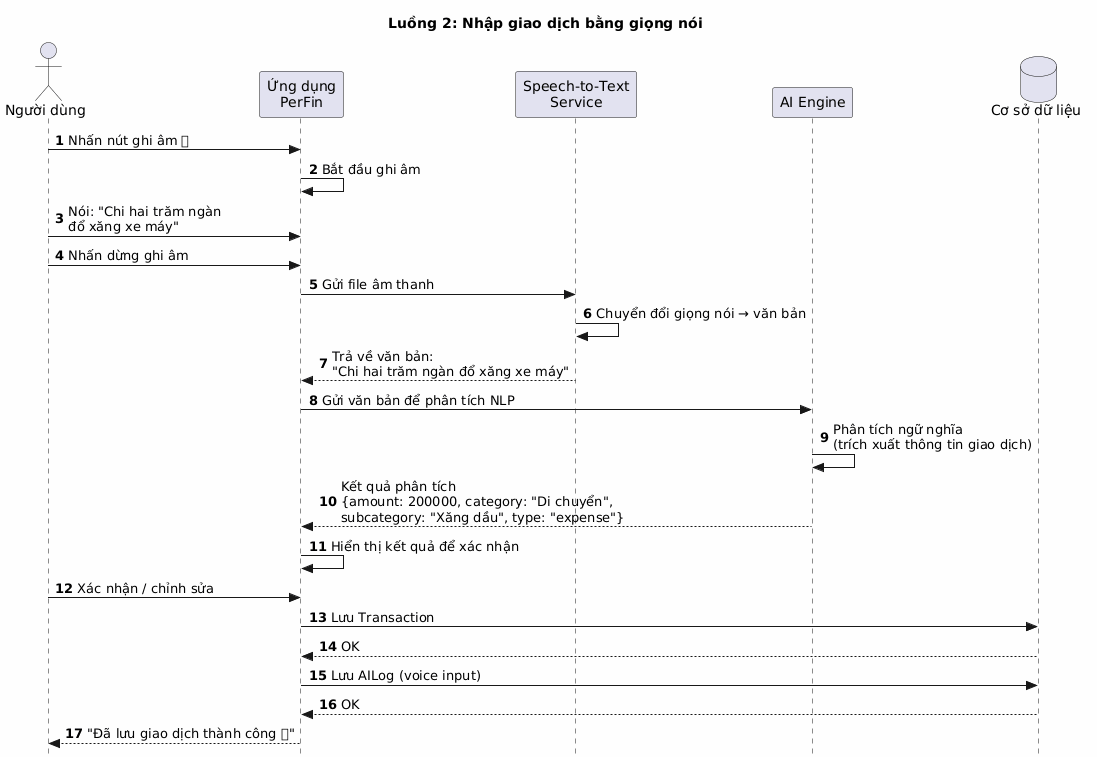
\includegraphics[width=0.9\textwidth]{images/sequence-nhập-giao-dịch-bằng-giọng-nói.png}
    \caption{Sơ đồ tuần tự: Nhập giao dịch bằng giọng nói}
    \label{fig:seq_voice_input}
\end{figure}

\begin{figure}[htbp]
    \centering
    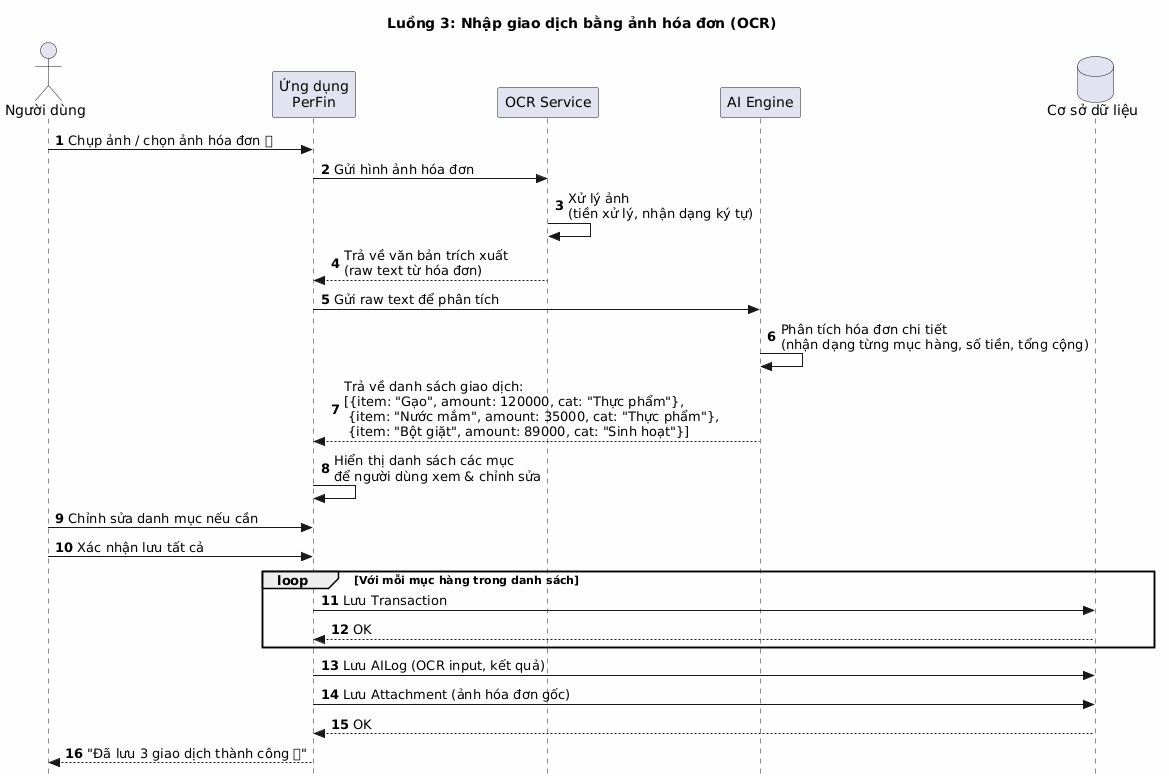
\includegraphics[width=0.9\textwidth]{images/sequence-nhập-giao-dịch-bằng-ảnh-hóa-đơn-ocr.png}
    \caption{Sơ đồ tuần tự: Nhập giao dịch bằng ảnh hóa đơn (OCR)}
    \label{fig:seq_ocr_input}
\end{figure}

\begin{figure}[htbp]
    \centering
    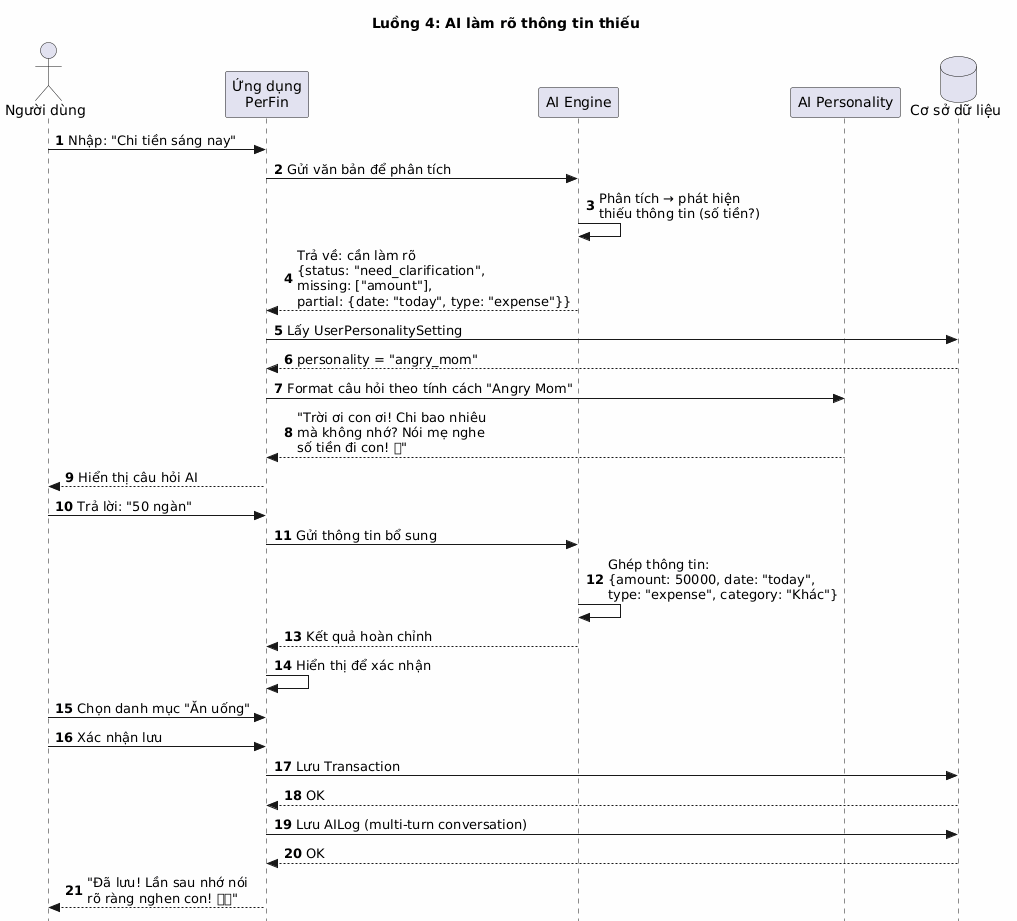
\includegraphics[width=0.9\textwidth]{images/sequence-ai-làm-rõ-thông-tin-thiếu.png}
    \caption{Sơ đồ tuần tự: AI làm rõ thông tin thiếu}
    \label{fig:seq_ai_clarify}
\end{figure}

\begin{figure}[htbp]
    \centering
    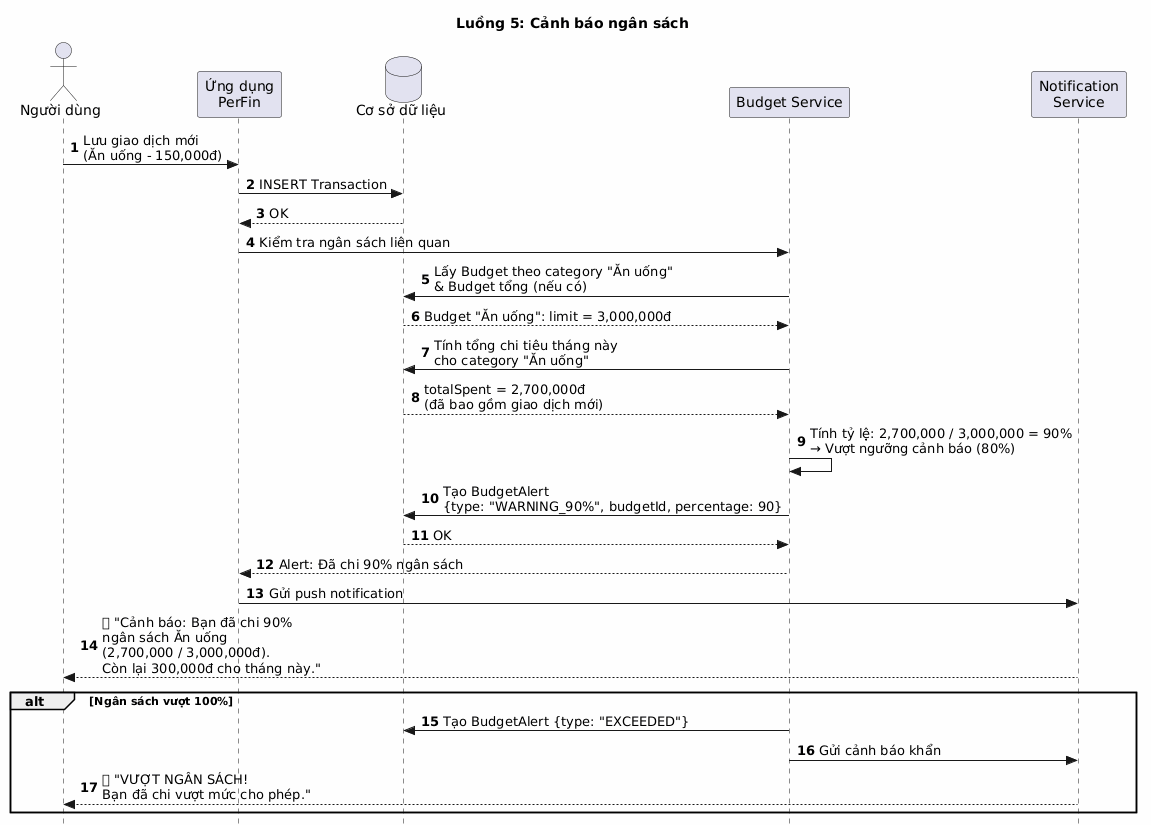
\includegraphics[width=0.9\textwidth]{images/sequence-cảnh-báo-ngân-sách.png}
    \caption{Sơ đồ tuần tự: Cảnh báo ngân sách}
    \label{fig:seq_budget_alert}
\end{figure}

\begin{figure}[htbp]
    \centering
    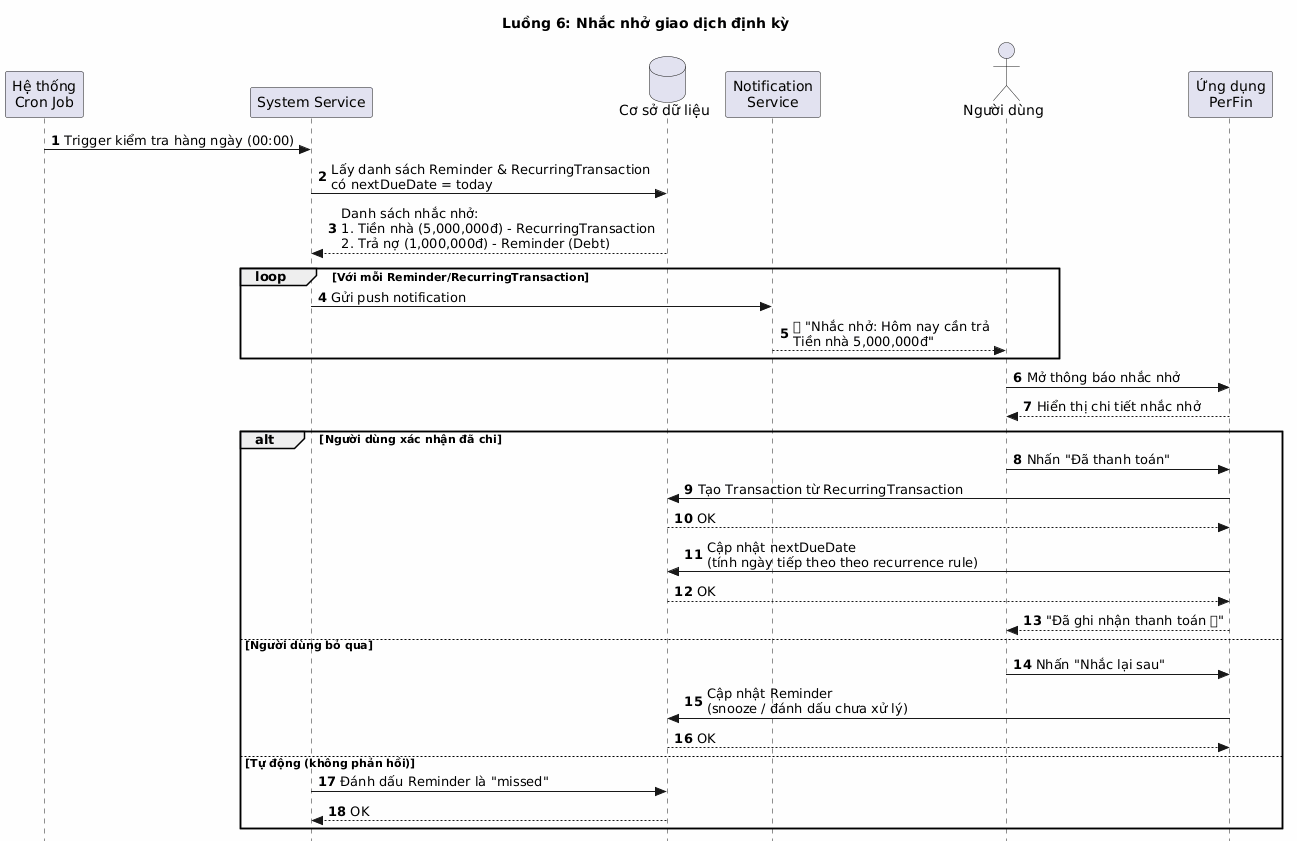
\includegraphics[width=0.9\textwidth]{images/sequence-nhắc-nhở-giao-dịch-định-kỳ.png}
    \caption{Sơ đồ tuần tự: Nhắc nhở giao dịch định kỳ}
    \label{fig:seq_recurring_reminder}
\end{figure}

\begin{figure}[htbp]
    \centering
    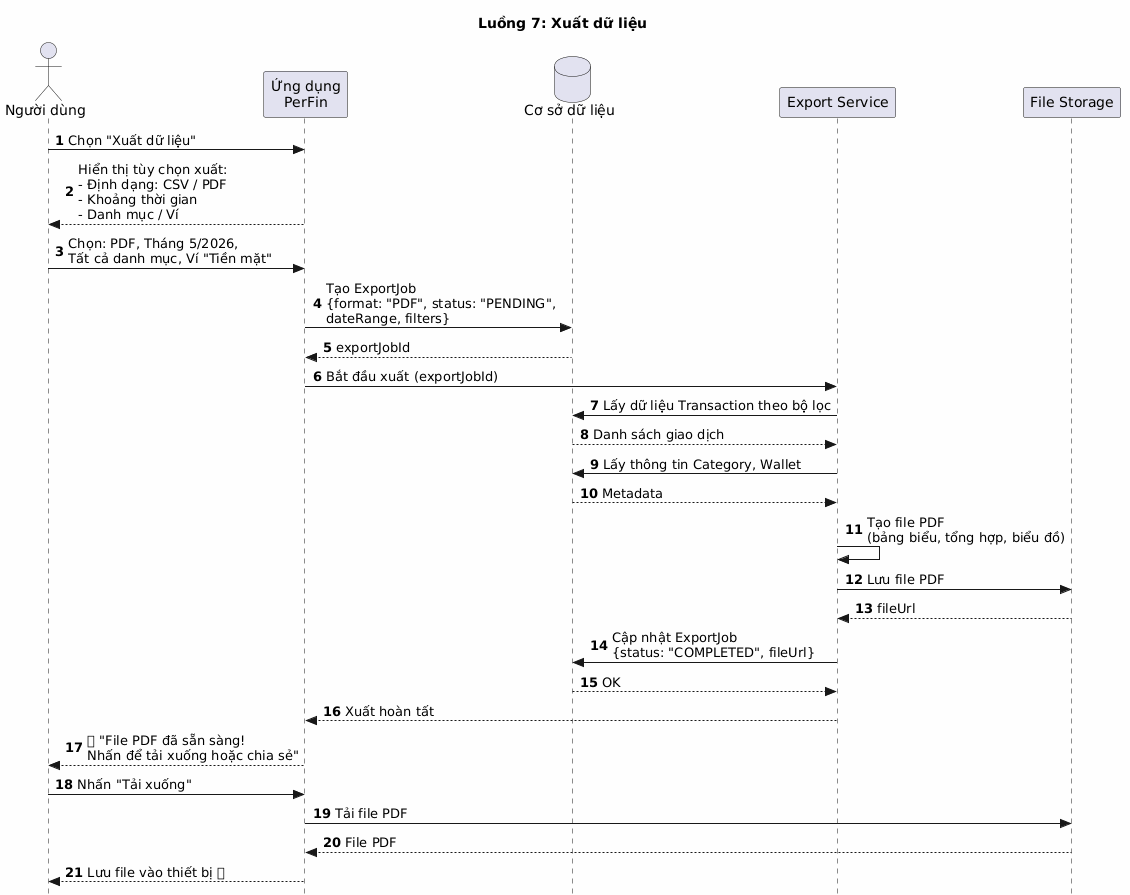
\includegraphics[width=0.9\textwidth]{images/sequence-xuất-dữ-liệu.png}
    \caption{Sơ đồ tuần tự: Xuất dữ liệu}
    \label{fig:seq_export_data}
\end{figure}

\begin{figure}[htbp]
    \centering
    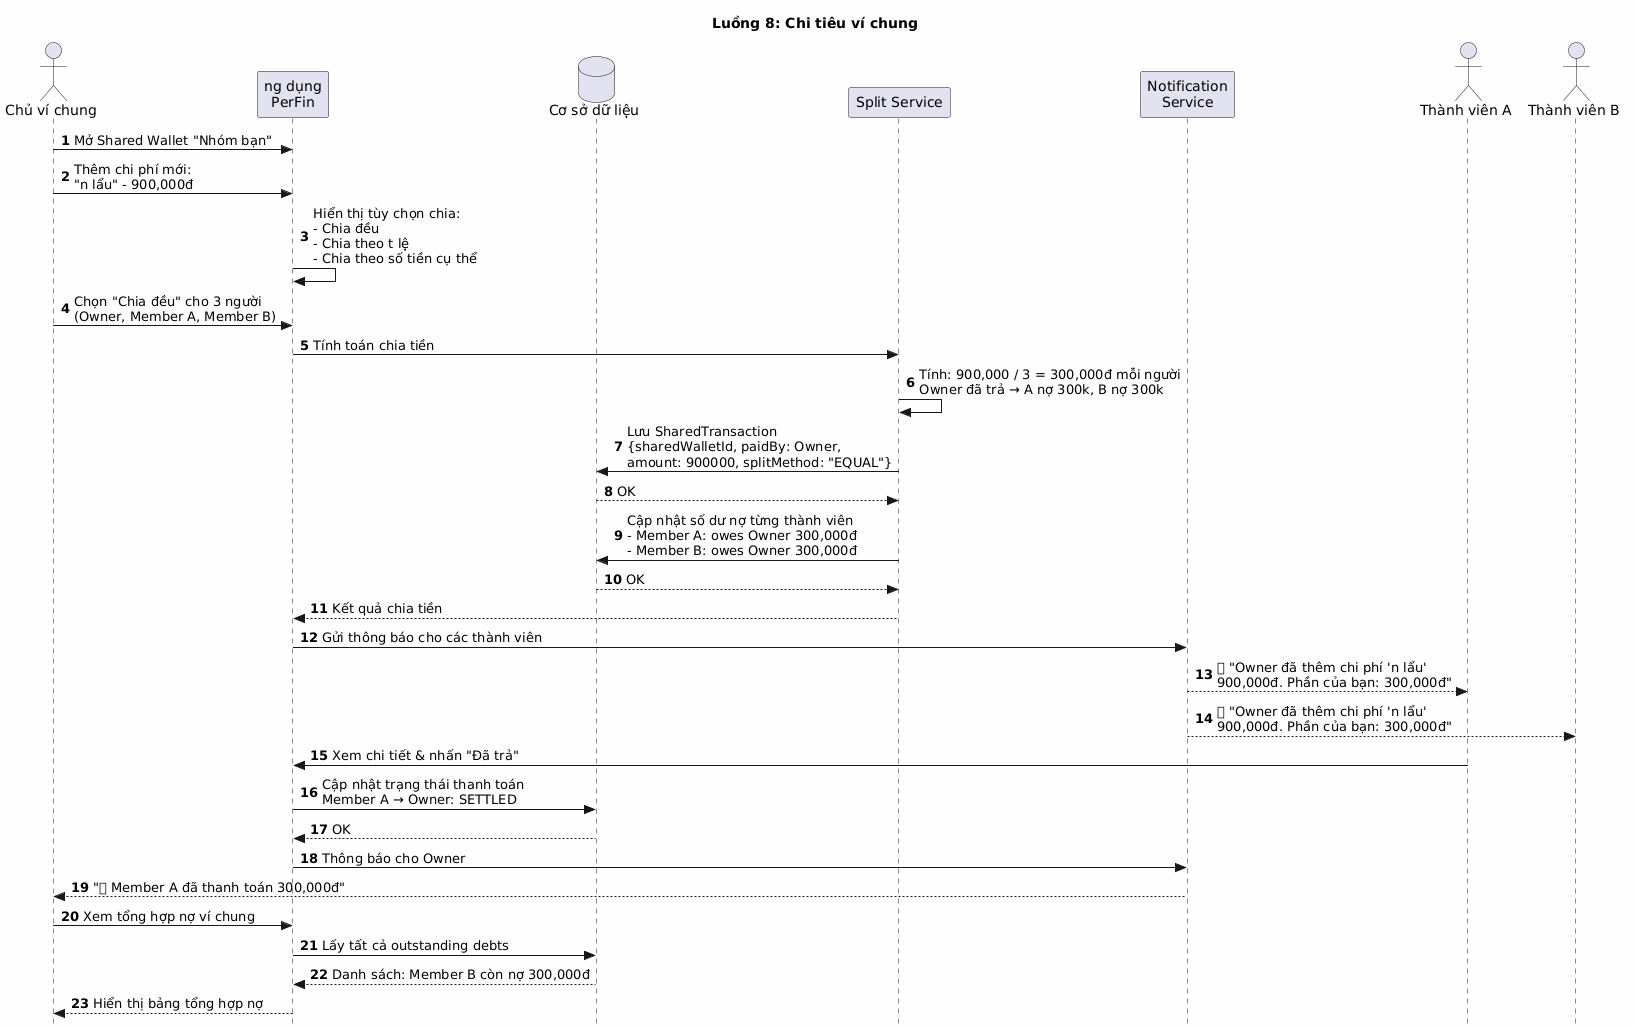
\includegraphics[width=0.9\textwidth]{images/sequence-chi-tiêu-ví-chung.png}
    \caption{Sơ đồ tuần tự: Chi tiêu ví chung}
    \label{fig:seq_shared_wallet}
\end{figure}

Dưới đây là mô tả 3 luồng tương tác quan trọng nhất trong hệ thống:

\begin{enumerate}
    \item \textbf{Nhập giao dịch bằng văn bản (Hình~\ref{fig:seq_text_input}):} Người dùng gửi tin nhắn dạng văn bản tự nhiên (ví dụ: ``trà sữa 50k'') qua Chat UI. Client gửi yêu cầu đến API Gateway, Gateway xác minh JWT token rồi chuyển tiếp đến AI Service. AI Service điều phối NLP Engine (Google Gemini API) để phân tích ngữ nghĩa, trích xuất intent (tạo giao dịch chi), entity (tên=``trà sữa'', số tiền=50.000đ), đồng thời Categorization Engine suy đoán danh mục phù hợp (``Ăn uống''). Kết quả trả về Transaction Service để tạo giao dịch mới trong Database, cập nhật số dư Wallet, và kiểm tra ngưỡng Budget. Phản hồi xác nhận được Personality Engine định dạng theo nhân cách AI đã chọn rồi trả về cho người dùng.

    \item \textbf{Nhập giao dịch bằng ảnh hóa đơn --- OCR (Hình~\ref{fig:seq_ocr_input}):} Người dùng chụp ảnh hóa đơn và gửi qua Chat UI. API Gateway chuyển ảnh đến AI Service, AI Service gọi OCR Engine (Google Vision API) để nhận dạng văn bản trong ảnh. Kết quả OCR (raw text) được chuyển tiếp cho NLP Engine để phân tích cấu trúc hóa đơn, trích xuất danh sách sản phẩm, đơn giá, và tổng tiền. Nếu thông tin đầy đủ, Transaction Service tạo giao dịch; nếu thiếu thông tin (ví dụ không xác định được danh mục), AI hỏi lại người dùng qua chat (xem Hình~\ref{fig:seq_ai_clarify}).

    \item \textbf{Cảnh báo ngân sách (Hình~\ref{fig:seq_budget_alert}):} Sau khi một Transaction mới được tạo thành công, Transaction Service phát sự kiện (event) đến Budget Service. Budget Service tính tổng chi tiêu hiện tại trong kỳ cho danh mục tương ứng, so sánh với hạn mức đã thiết lập. Khi tổng chi tiêu vượt các ngưỡng cảnh báo (70\%, 90\%, hoặc 100\% hạn mức), Budget Service gửi yêu cầu đến Notification Service để tạo cảnh báo. Notification Service gửi thông báo đẩy (push notification) và hiển thị cảnh báo trong giao diện chat để người dùng kịp thời điều chỉnh hành vi chi tiêu.
\end{enumerate}

\subsubsection{Sơ đồ hoạt động (Activity Diagrams)}
Các sơ đồ hoạt động mô tả chi tiết quy trình xử lý cho các luồng nghiệp vụ phức tạp.

Các sơ đồ hoạt động mô tả chi tiết quy trình xử lý và logic nghiệp vụ bên trong hệ thống cho các tính năng phức tạp:

\begin{figure}[htbp]
    \centering
    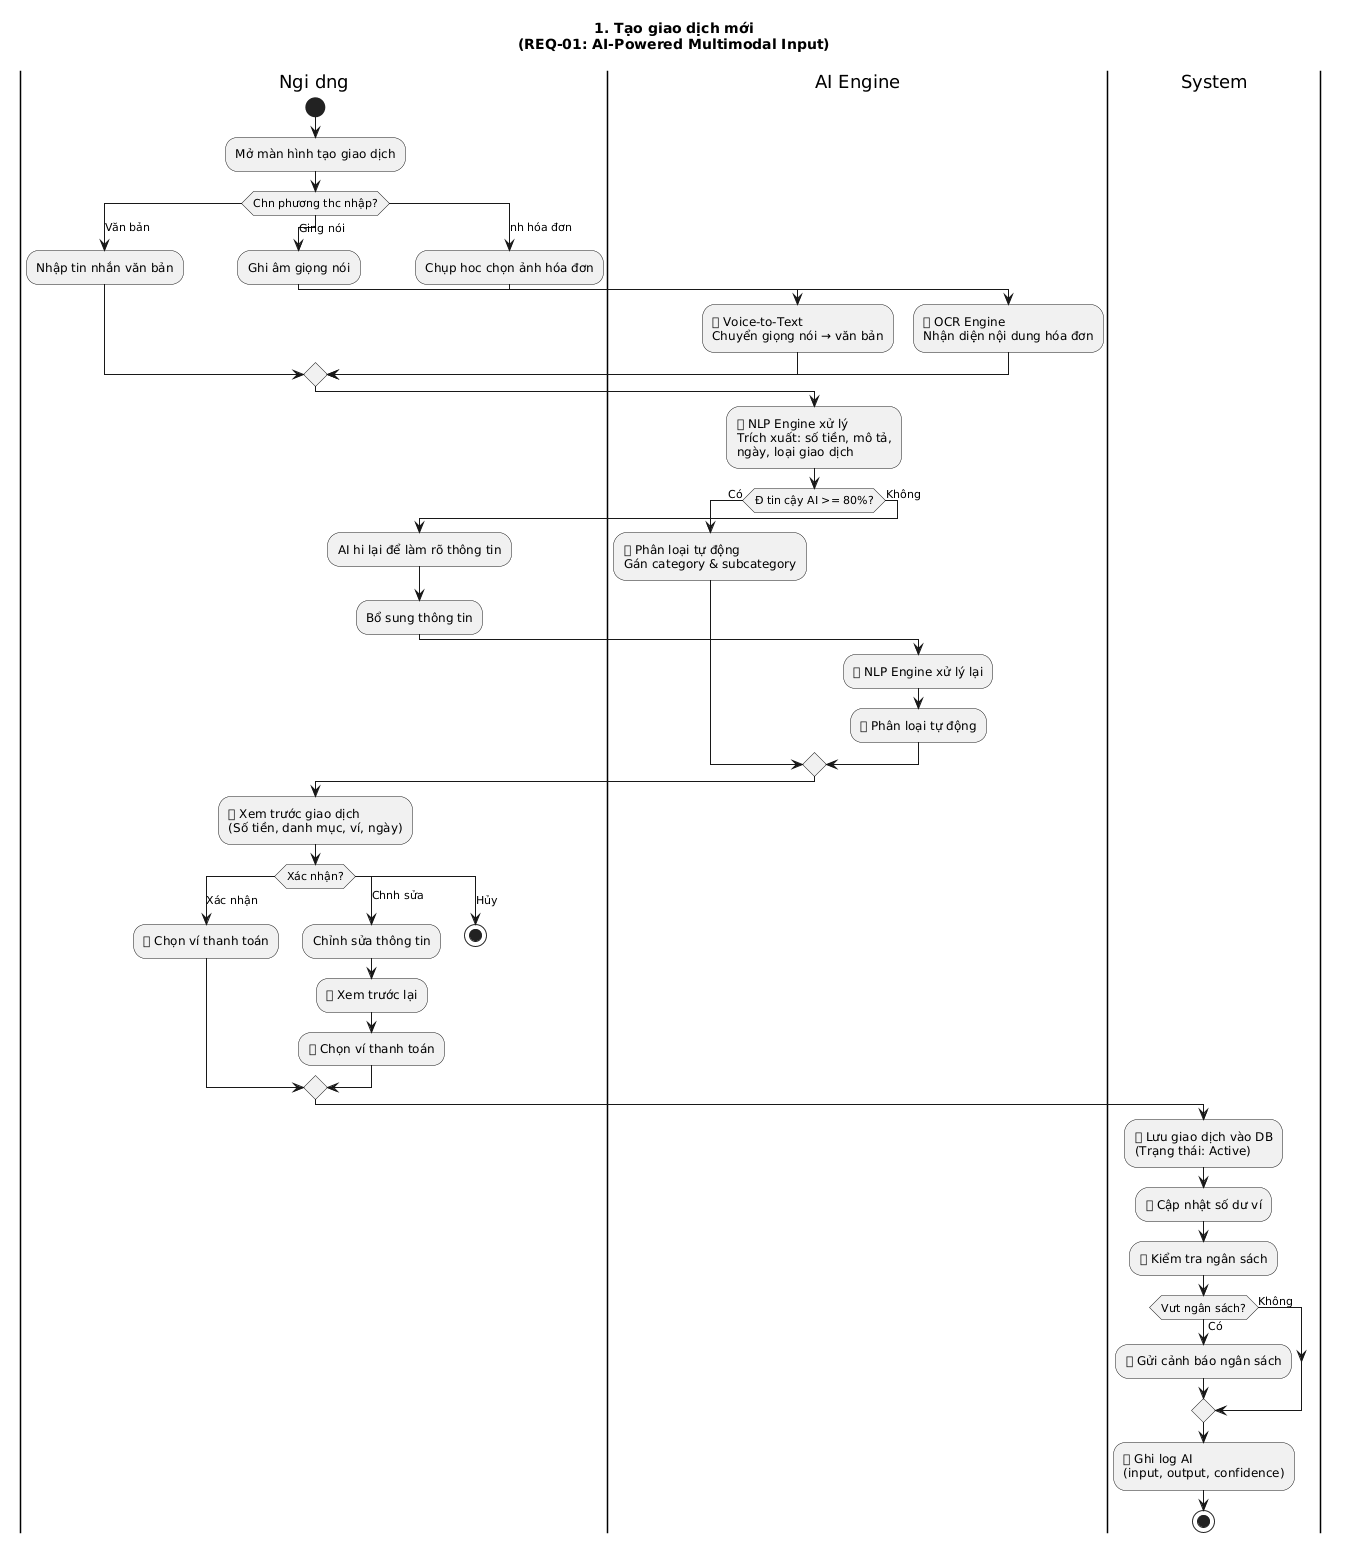
\includegraphics[width=0.85\textwidth]{images/activity-tạo-giao-dịch-mớinreq-01-ai-powered-multimodal-input.png}
    \caption{Sơ đồ hoạt động: Tạo giao dịch mới (REQ-01)}
    \label{fig:act_create_trans}
\end{figure}

\begin{figure}[htbp]
    \centering
    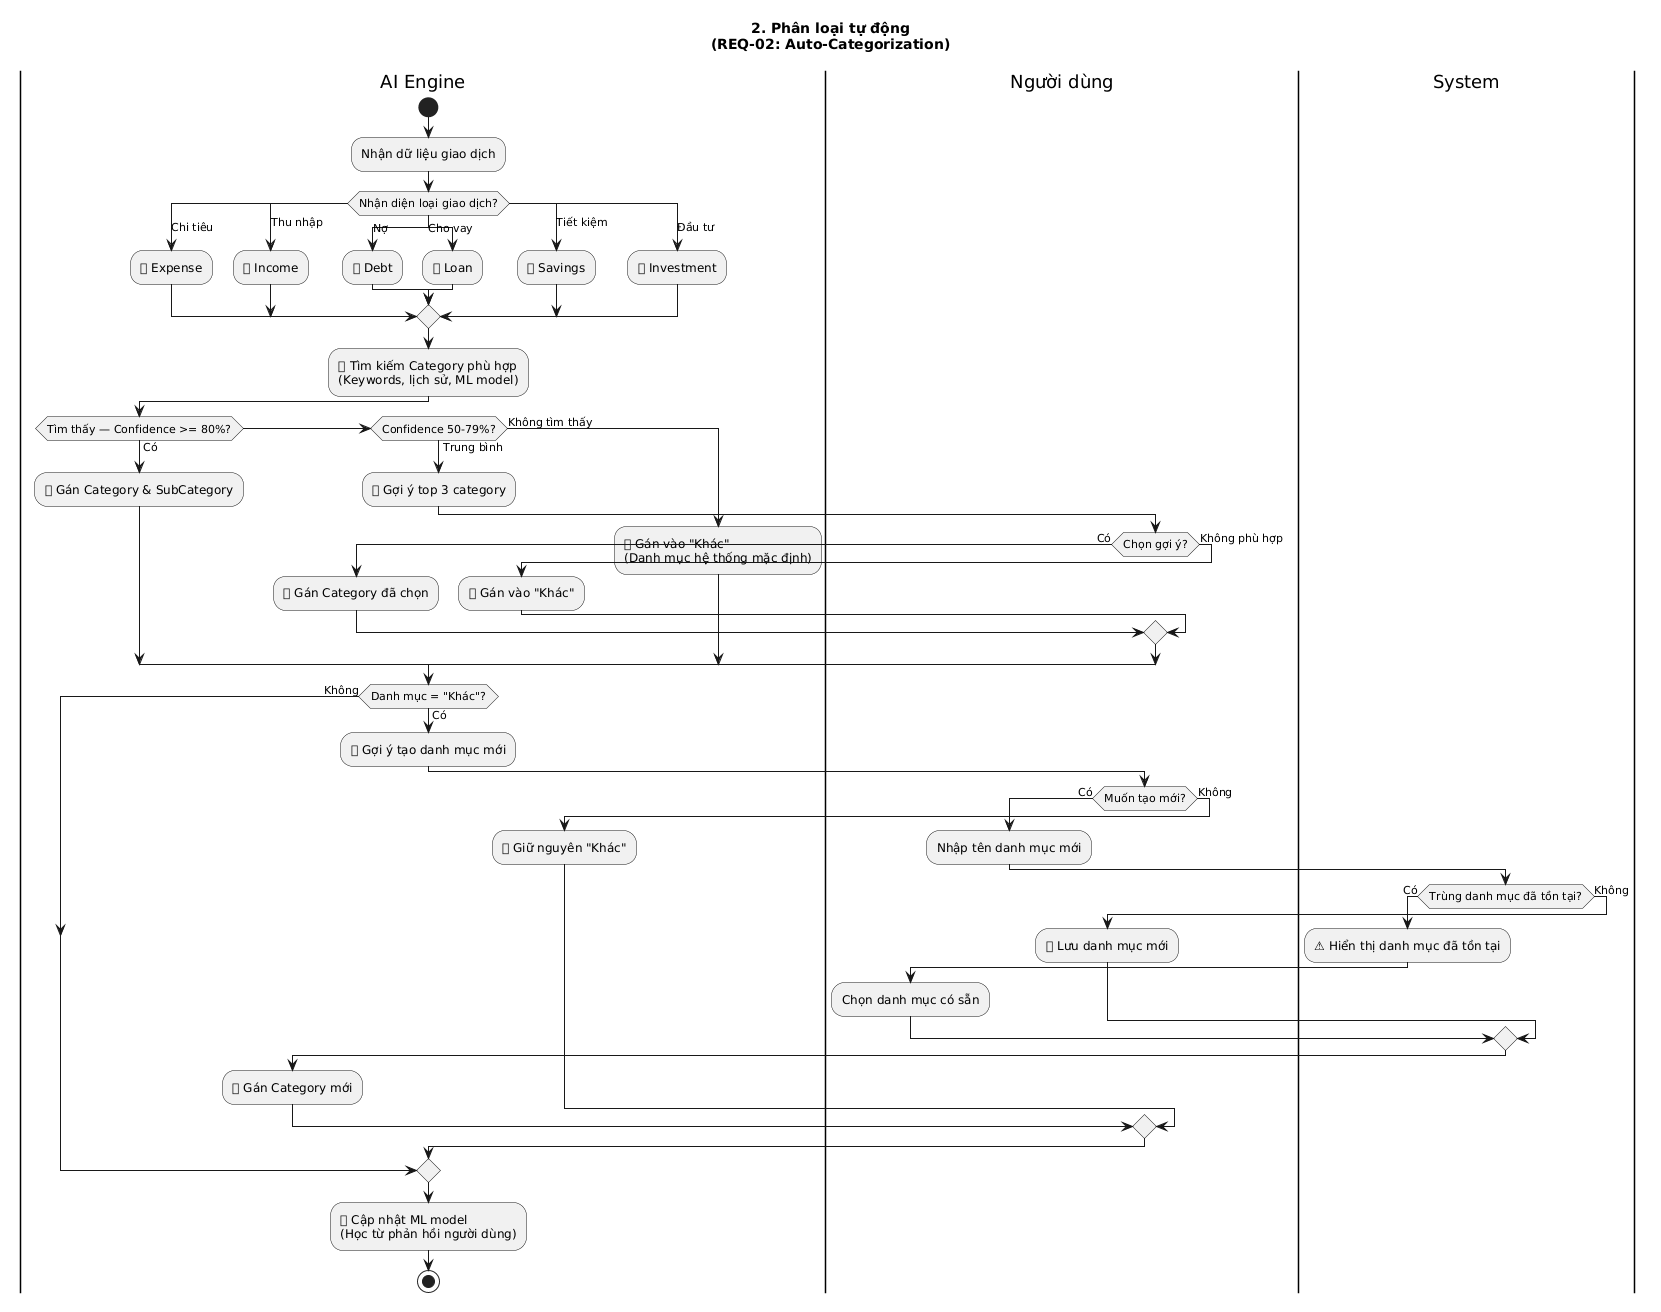
\includegraphics[width=0.85\textwidth]{images/activity-phân-loại-tự-độngnreq-02-auto-categorization.png}
    \caption{Sơ đồ hoạt động: Phân loại tự động (REQ-02)}
    \label{fig:act_auto_cat}
\end{figure}

\begin{figure}[htbp]
    \centering
    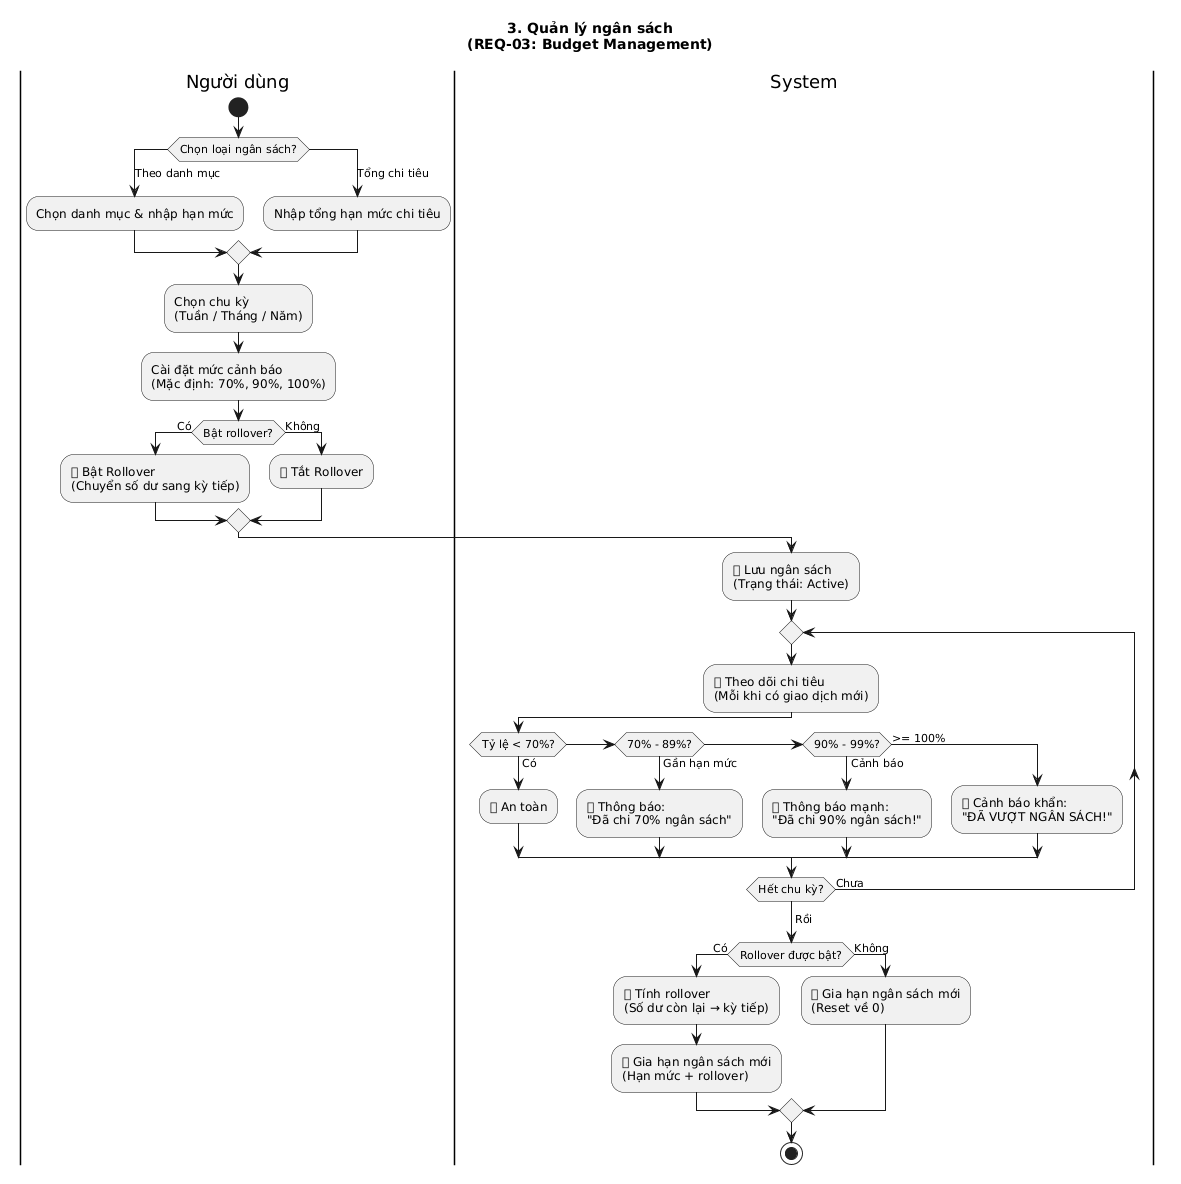
\includegraphics[width=0.85\textwidth]{images/activity-quản-lý-ngân-sáchnreq-03-budget-management.png}
    \caption{Sơ đồ hoạt động: Quản lý ngân sách (REQ-03)}
    \label{fig:act_budget_mgmt}
\end{figure}

\begin{figure}[htbp]
    \centering
    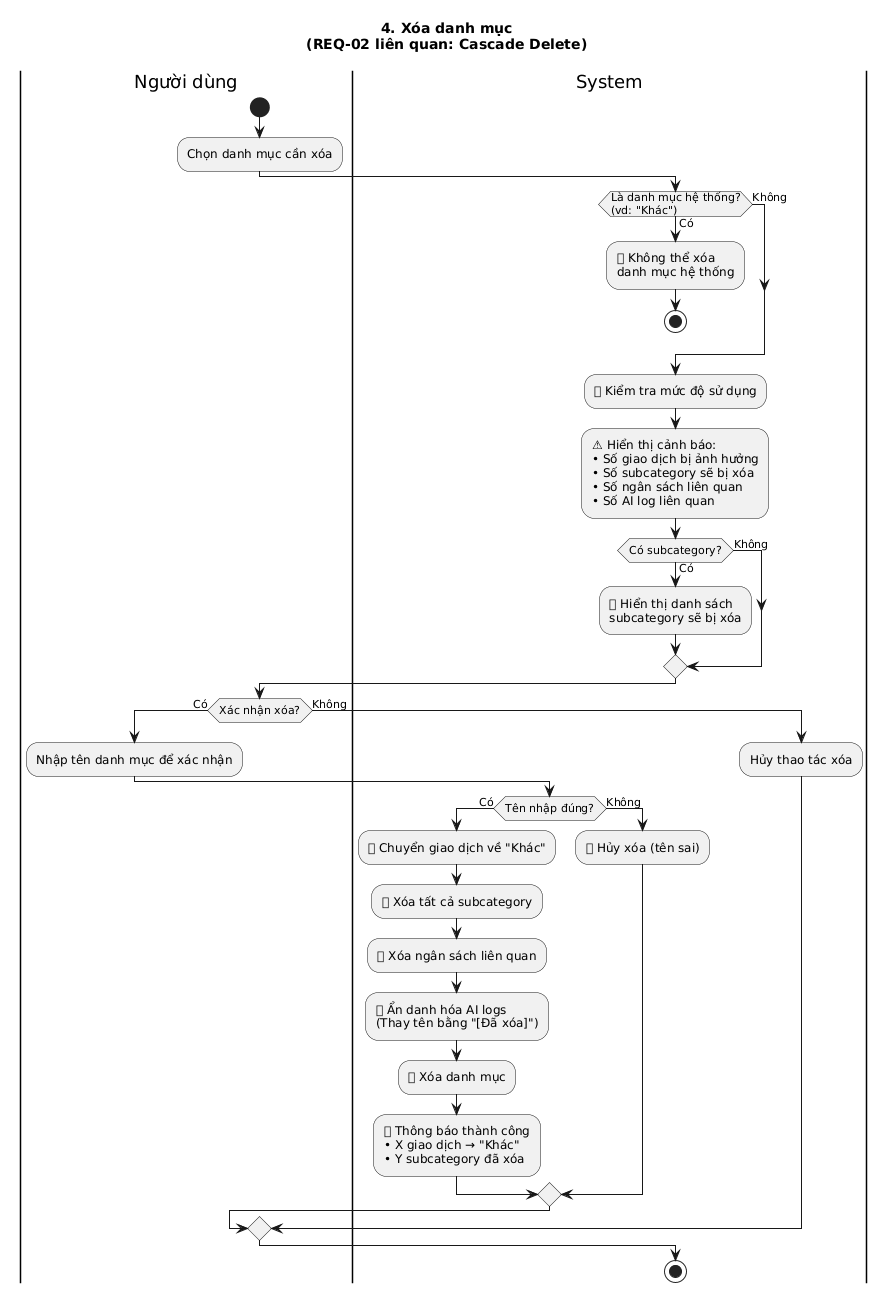
\includegraphics[width=0.85\textwidth]{images/activity-xóa-danh-mụcnreq-02-liên-quan-cascade-delete.png}
    \caption{Sơ đồ hoạt động: Xóa danh mục (REQ-02)}
    \label{fig:act_delete_cat}
\end{figure}

\begin{figure}[htbp]
    \centering
    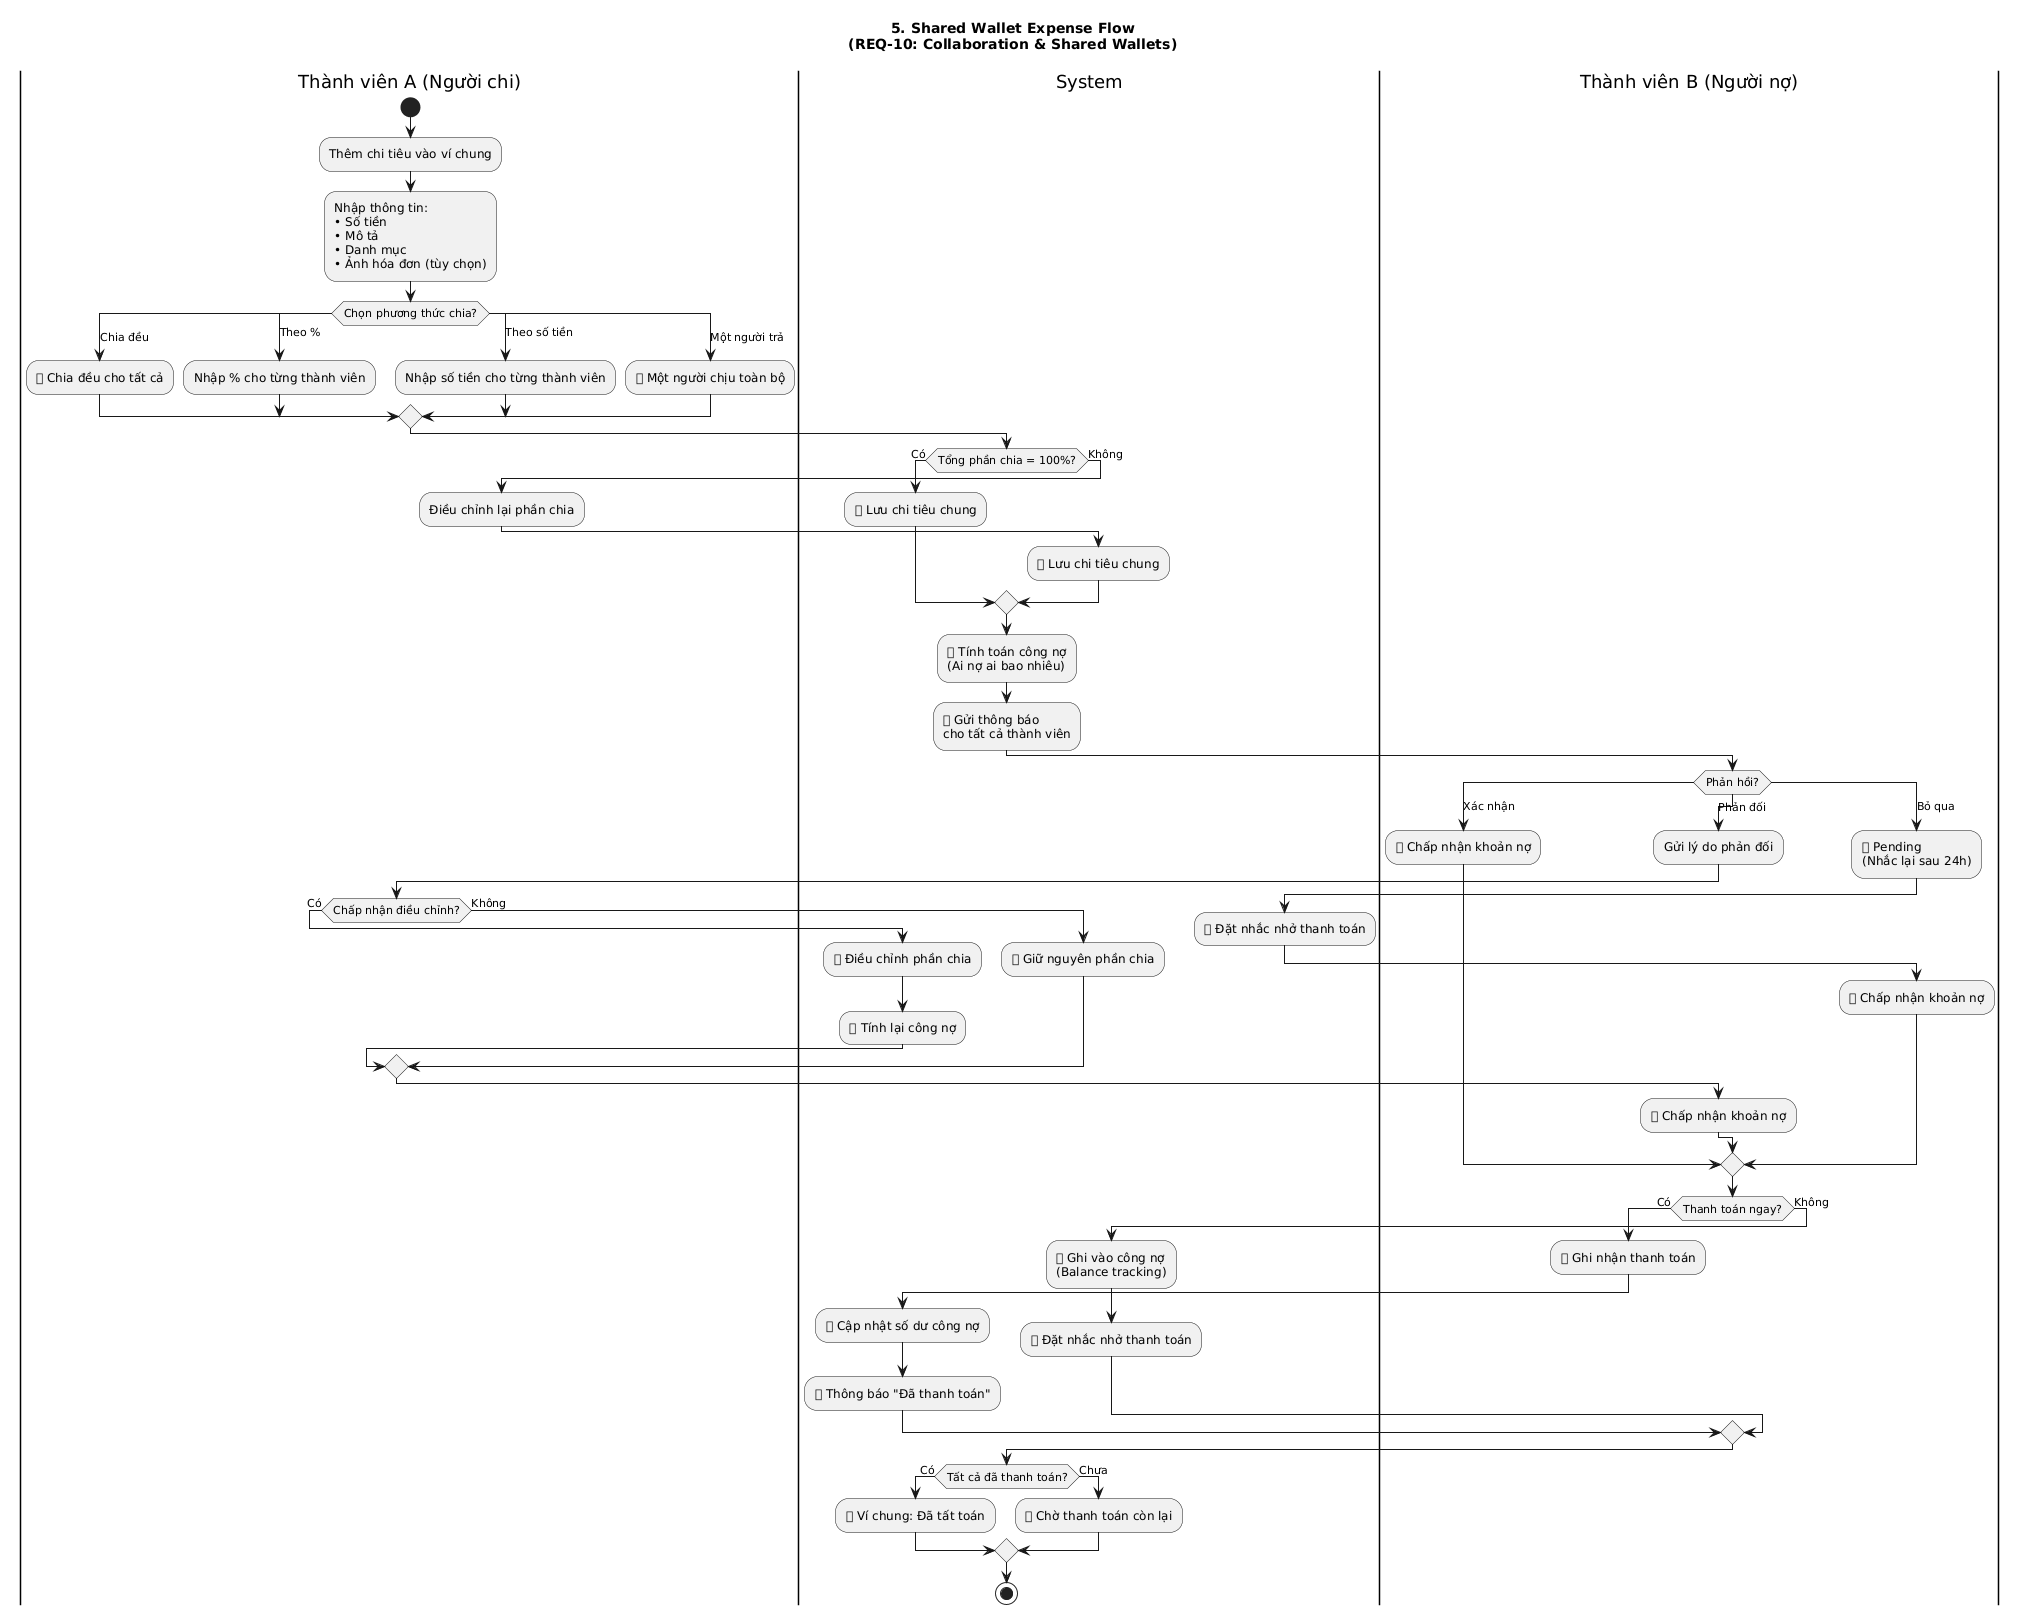
\includegraphics[width=0.85\textwidth]{images/activity-shared-wallet-expense-flownreq-10-collaboration-shared-wallets.png}
    \caption{Sơ đồ hoạt động: Quy trình chi tiêu ví chung (REQ-10)}
    \label{fig:act_shared_wallet}
\end{figure}

Dưới đây là mô tả các quy trình xử lý chính được thể hiện trong các sơ đồ hoạt động:

\begin{enumerate}
    \item \textbf{Luồng tạo giao dịch mới (Hình~\ref{fig:act_create_trans}):} Quy trình bắt đầu khi hệ thống nhận đầu vào từ người dùng. Bước đầu tiên là xác định loại đầu vào: văn bản (text), giọng nói (voice), hoặc hình ảnh (image). Nếu là giọng nói, hệ thống chuyển đổi thành văn bản qua Voice-to-Text Engine; nếu là hình ảnh, hệ thống trích xuất văn bản qua OCR Engine. Sau đó, NLP Engine phân tích ngữ nghĩa văn bản để trích xuất thông tin giao dịch (tên, số tiền, ngày). Categorization Engine suy đoán danh mục phù hợp dựa trên ngữ cảnh và lịch sử. Nếu thông tin đầy đủ và AI có độ tin cậy cao, hệ thống hiển thị kết quả để người dùng xác nhận; nếu thiếu thông tin, AI hỏi lại. Cuối cùng, giao dịch được lưu vào cơ sở dữ liệu và số dư ví được cập nhật.

    \item \textbf{Luồng phân loại tự động (Hình~\ref{fig:act_auto_cat}):} Khi nhận được nội dung giao dịch cần phân loại, Categorization Engine thực hiện phân tích ngữ cảnh (context analysis) dựa trên từ khóa, mô tả giao dịch, và lịch sử phân loại của người dùng. Hệ thống tra cứu danh sách danh mục hiện có (cả mặc định và tùy chỉnh), tính toán độ tin cậy (confidence score) cho danh mục phù hợp nhất. Nếu confidence $\ge$ ngưỡng cấu hình (mặc định 85\%), hệ thống tự động gán danh mục; nếu confidence thấp hơn, hệ thống đề xuất danh mục kèm theo câu hỏi xác nhận từ người dùng. Phản hồi của người dùng (chấp nhận hoặc chọn danh mục khác) được ghi nhận để cải thiện độ chính xác cho các lần phân loại sau (feedback loop).

    \item \textbf{Luồng quản lý ngân sách (Hình~\ref{fig:act_budget_mgmt}):} Quy trình bắt đầu khi người dùng thiết lập ngân sách cho một danh mục trong kỳ (tuần/tháng). Mỗi khi giao dịch mới được tạo, hệ thống tự động tính toán tổng chi tiêu hiện tại so với hạn mức. Tại các ngưỡng 70\%, 90\%, và 100\%, hệ thống kích hoạt cảnh báo tương ứng. Khi kết thúc kỳ, nếu ngân sách chưa dùng hết và tùy chọn rollover được bật, phần dư sẽ được chuyển sang kỳ tiếp theo.
\end{enumerate}

\subsubsection{Thiết kế giao diện người dùng (UI Design)}
[TODO --- Trình bày wireframe/mockup cho các màn hình chính:
\begin{enumerate}
    \item Màn hình Chat (giao diện chính)
    \item Màn hình Dashboard/Tổng quan
    \item Màn hình Báo cáo/Biểu đồ
    \item Màn hình Quản lý Ngân sách
    \item Màn hình Quản lý Ví/Tài khoản
    \item Màn hình Cài đặt
\end{enumerate}
]

\subsubsection{Mô tả thuật toán và kỹ thuật quan trọng}
[TODO --- Giải thích chi tiết:
\begin{enumerate}
    \item Luồng xử lý NLP: từ input text $\rightarrow$ intent classification $\rightarrow$ entity extraction $\rightarrow$ transaction creation
    \item Luồng xử lý OCR: từ image $\rightarrow$ preprocessing $\rightarrow$ text detection $\rightarrow$ structured data extraction
    \item Thuật toán phân loại danh mục: prompt engineering cho LLM, feedback loop
    \item Thuật toán phát hiện bất thường chi tiêu
    \item Cơ chế cảnh báo ngân sách proactive
\end{enumerate}
]

\section{Kiểm thử (Testing)}
\label{sec:testing}

\subsection{Kế hoạch kiểm thử (Test Plan)}
\label{subsec:test_plan}

Chiến lược kiểm thử của PerFin được xây dựng theo mô hình kim tự tháp kiểm thử (Testing Pyramid), trong đó Unit Testing chiếm tỷ trọng lớn nhất, tiếp theo là Integration Testing, System Testing, và cuối cùng là User Acceptance Testing. Các loại kiểm thử cụ thể:

\subsubsection{Các loại kiểm thử}

\begin{table}[htbp]
\centering
\begin{tabularx}{\textwidth}{|l|X|l|}
\hline
\textbf{Loại kiểm thử} & \textbf{Mô tả} & \textbf{Công cụ} \\ \hline
Unit Testing & Kiểm thử từng hàm/module riêng lẻ, đặc biệt các hàm xử lý logic nghiệp vụ (tính toán số dư, kiểm tra ngưỡng ngân sách) và các hàm tiện ích (format tiền tệ, parse ngày tháng) & Jest (Node.js), Flutter Test \\ \hline
Integration Testing & Kiểm thử tích hợp giữa các service, đảm bảo API endpoint hoạt động đúng với request/response, kiểm tra luồng dữ liệu giữa các tầng & Supertest, Postman \\ \hline
System Testing & Kiểm thử toàn hệ thống end-to-end, mô phỏng luồng sử dụng thực tế từ giao diện mobile đến database & Appium, Flutter Driver \\ \hline
User Acceptance Testing & Kiểm thử chấp nhận với 5--10 người dùng thực thuộc nhóm đối tượng mục tiêu (sinh viên, người đi làm trẻ), đánh giá tính dễ sử dụng và độ chính xác AI & Manual Testing \\ \hline
\end{tabularx}
\caption{Kế hoạch kiểm thử}
\label{tab:test_plan}
\end{table}

\subsubsection{Các test case chính}

Bảng~\ref{tab:test_cases} liệt kê các test case cho các luồng nghiệp vụ quan trọng nhất của hệ thống:

\begin{table}[htbp]
\centering
\begin{tabularx}{\textwidth}{|l|p{3.5cm}|X|p{2cm}|p{2cm}|p{1.5cm}|}
\hline
\textbf{Mã TC} & \textbf{Mô tả} & \textbf{Đầu vào} & \textbf{Kết quả mong đợi} & \textbf{Kết quả thực tế} & \textbf{Trạng thái} \\ \hline
TC-01 & Nhập giao dịch bằng văn bản tiếng Việt & "trà sữa 50k" & Tạo giao dịch: tên="trà sữa", số tiền=50.000đ, danh mục="Ăn uống" & [TODO] & [TODO] \\ \hline
TC-02 & Nhập giao dịch bằng hình ảnh hóa đơn & Ảnh hóa đơn siêu thị & Trích xuất danh sách sản phẩm và tổng tiền & [TODO] & [TODO] \\ \hline
TC-03 & Cảnh báo ngân sách 70\% & Chi tiêu vượt 70\% hạn mức & Hệ thống gửi cảnh báo trong chat & [TODO] & [TODO] \\ \hline
TC-04 & Phân loại tự động & "grab đi làm 30k" & Giao dịch phân loại vào "Di chuyển" & [TODO] & [TODO] \\ \hline
TC-05 & Nhập giao dịch bằng giọng nói & "mua cà phê ba mươi nghìn" (voice) & Tạo giao dịch: tên="cà phê", số tiền=30.000đ, danh mục="Ăn uống" & [TODO] & [TODO] \\ \hline
TC-06 & Chuyển tiền giữa ví & "chuyển 500k từ tiền mặt sang Momo" & Tạo Transfer, số dư tiền mặt giảm 500.000đ, số dư Momo tăng 500.000đ & [TODO] & [TODO] \\ \hline
TC-07 & Xem báo cáo chi tiêu tháng & Yêu cầu xem báo cáo tháng 6 & Hiển thị biểu đồ tròn theo danh mục, tổng thu/chi chính xác & [TODO] & [TODO] \\ \hline
TC-08 & Đổi nhân cách AI & Chọn nhân cách ``Bà mẹ nghiêm khắc'' & Giọng điệu chat thay đổi phù hợp, logic xử lý giao dịch không đổi & [TODO] & [TODO] \\ \hline
TC-09 & Xuất dữ liệu CSV & Yêu cầu xuất giao dịch 3 tháng gần nhất & File CSV tải về thành công, dữ liệu đầy đủ và đúng định dạng & [TODO] & [TODO] \\ \hline
TC-10 & Sao lưu dữ liệu & Yêu cầu sao lưu toàn bộ dữ liệu & File backup mã hóa AES-256 được tạo thành công & [TODO] & [TODO] \\ \hline
\end{tabularx}
\caption{Các test case chính}
\label{tab:test_cases}
\end{table}

\subsection{Kết quả và phân tích (Results \& Analysis)}
\label{subsec:test_results}

[TODO --- Trình bày kết quả kiểm thử và sử dụng bảng, biểu đồ để minh họa:
\begin{itemize}
    \item Tỷ lệ pass/fail của test case
    \item Độ chính xác phân loại danh mục
    \item Thời gian phản hồi trung bình
    \item Kết quả UAT
\end{itemize}
]
